\documentclass[12pt]{article}
\pdfoutput=1

\usepackage{graphics,amssymb,float}
%\usepackage[usenames,dvips]{color}
\usepackage{graphicx}% Include figure files
\usepackage{subfigure}
\usepackage{color}
\usepackage{xspace}
\usepackage{placeins}
%\usepackage[color]{showkeys}
%\usepackage{epsfig}% Include figure files
\usepackage{rotating}% Include figure files
\usepackage{dcolumn}% Align table columns on decimal point
\usepackage{bm}% bold math
\usepackage{cite}
\usepackage{amsmath}
\usepackage{indentfirst} % activate indent in the first paragraph
\usepackage{epstopdf}
\usepackage{tikz}
\usetikzlibrary{shapes,arrows}

\bibliographystyle{utphys}


\textheight=22.8 truecm
\textwidth=17 truecm
\topmargin=-3mm
\voffset=-1 truecm
\hoffset=-2 truecm

\def\eg{{\it e.g.}}
\def\ie{{\it i.e.}}
\def\mgut{M_{\rm GUT}}

\def\Eq#1{Eq.~(\ref{#1})}
%\def\Eqs#2{Eqs.~(\ref{#1})--\ref{#2})}

\def\lsim{\mathrel{\raise.3ex\hbox{$<$\kern-.75em\lower1ex\hbox{$\sim$}}}}
\def\gsim{\mathrel{\raise.3ex\hbox{$>$\kern-.75em\lower1ex\hbox{$\sim$}}}}
\def\ifmath#1{\relax\ifmmode #1\else $#1$\fi}

\def\change{\marginpar{\bf text changed}}
\def\new{\marginpar{\bf new addition}}
\def\check{\marginpar{\bf check!}}

\begin{document}
%\begin{titlepage}
\begin{center}


%\vspace*{-1cm}
\begin{flushright}
preprint numbers
%LAPTH-061/12\\
%LPSC12350\\
%LPT Orsay 12-119\\
%NSF-KITP-12-236
\end{flushright}

\vspace*{1.6cm}
{\Large\bf A survey of supersymmetry\\[3mm] based on simplified-model results from the LHC} 

\vspace*{1cm}\renewcommand{\thefootnote}{\fnsymbol{footnote}}

{\large 
%B.~Dumont$^{1}$\footnote[2]{Email: dumont@lpsc.in2p3.fr},
Sabine~Kraml$^{1}$\footnote[1]{Email: sabine.kraml@lpsc.in2p3.fr},
Suchita~Kulkarni$^{1}$\footnote[2]{Email: suchita.kulkarni@lpsc.in2p3.fr},
Wolfgang Waltenberger$^{2}$\footnote[3]{Email: wolfgang.waltenberger@oeaw.ac.at}
} 

\renewcommand{\thefootnote}{\arabic{footnote}}

\vspace*{1cm} 
{\normalsize \it 
$^1\,$Laboratoire de Physique Subatomique et de Cosmologie, UJF Grenoble 1,
CNRS/IN2P3, INPG, 53 Avenue des Martyrs, F-38026 Grenoble, France\\[2mm]
$^2\,$Institut f\"ur Hochenergiephysik,  \"Osterreichische Akademie der Wissenschaften,\\ Nikolsdorfer Gasse 18, 1050 Wien, Austria\\[1mm]
}

\vspace{1cm}

\begin{abstract}
  Abstract
\end{abstract}

\end{center}

%\end{titlepage}


%%%%%%%%%%%%%%%%%%%%%%%%%%%%%%%%%%%%%%%%
\section{Introduction}
%%%%%%%%%%%%%%%%%%%%%%%%%%%%%%%%%%%%%%%%

Searches at the ATLAS and CMS experiments at the LHC show no signs of new physics whatsoever. 
After the first phase of LHC operation at centre-of-mass energies of 7--8~TeV in 2010--2012, 
the limits for the masses of supersymmetric particles, in particular of  squarks and gluinos, 
have been pushed well into the TeV range~\cite{atlas:susy:twiki,cms:susy:twiki}. 
%See \cite{atlas:susy:twiki,cms:susy:twiki} for the latest results.
Likewise, precision measurements in the flavor sector, in particular in $B$-physics, 
are well consistent with Standard Model (SM) expectations~\cite{Amhis:2012bh,lhcb:2012ct} 
and show no sign, or need, of new physics. 
At the same time the recent discovery~\cite{atlas:2012gk,cms:2012gu} of a Higgs-like particle 
with mass around 125~GeV makes the question of stability of the electroweak scale---the 
infamous gauge hierarchy problem---even  more imminent. 
Indeed, supersymmetry (SUSY) is arguably the best-motivated theory to solve the gauge 
hierarchy problem and to explain a light SM-like Higgs boson. 
So, the Higgs has very likely been discovered---but where is supersymmetry? 

Looking closely \cite{Sekmen:2011cz,Arbey:2011un,Papucci:2011wy,CahillRowley:2012kx,Dreiner:2012gx,Mahbubani:2012qq} 
one soon realizes that many of the current limits on SUSY particles are based 
on severe model assumptions, which impose particular relations between particle masses, decay 
branching rations, {\it etc}. The prime example is the interpretation of the search results within the 
Constrained Minimal Supersymmetric Standard Model (CMSSM). Another approach, which   
has become quite standard for the experiments, is to interpret the results 
within so-called Simplified Model Spectra \cite{Okawa:2011xg,cms:2013wc}.  
Simplified Model Spectra, or SMS for short, are effective-Lagrangian descriptions involving %the interactions of 
just a small number of new particles. They were designed as a useful tool for the characterization 
of new physics, see \eg\ \cite{Alwall:2008ag,Alves:2011wf}. 
On the whole, a large variety of results on searches in many different channels\footnote{Unfortunately with large variations in the level of documentation and details given on the analyses.} are available from both ATLAS and CMS, but it is quite difficult to determine whether a particular parameter point or scenario is allowed or excluded. 

In this paper, we present a method to decompose the signal of an arbitrary SUSY spectrum into simplified model  
topologies and thus test it against all the existing bounds derived in the SMS context. 
As we will show, this allows a vast survey of general and less general SUSY models, and enormously simplifies the task of designing the regions of parameter space which are still allowed, and/or have not yet been explored, by the current searches.
A scan over a 7-parameter realization of the MSSM is used as a show-case example to demonstrate the power of our method. 
Even in this example of limited complexity (as compared to, \eg, the 19-parameter phenomenological MSSM or the completely general MSSM with more than 100 free parameters) it turns out that large regions of interesting parameter space with SUSY particles below 1~TeV %survive the current bounds. 
remain unchallenged by the current bounds.

%The question what we really know about SUSY in general has been adressed in \cite{Sekmen:2011cz,Arbey:2011un,Papucci:2011wy,CahillRowley:2012kx} and some loopholes for evading the mainstream limits have been pointed out in, \eg, \cite{Dreiner:2012gx,Mahbubani:2012qq}. A recast of SMS limits onto minimal supergravity was attempted in \cite{Gutschow:2012pw}.

\subsection{Simplified models spectra and naming conventions}
\def\chitz{\ensuremath{\widetilde{\chi}^0_2}}
\def\chiz{\ensuremath{\widetilde{\chi}^0_1}}
\def\chipm{\ensuremath{\widetilde{\chi}^\pm_1}}
\def\chimp{\ensuremath{\widetilde{\chi}^\mp_1}}
\def\gl{\tilde{g}}
\def\sTop{\ensuremath{\tilde{t}}\xspace}
\def\st{\ensuremath{\tilde{t}}\xspace}
\def\slep{\ensuremath{\tilde{l}}\xspace}
\def\snu{\ensuremath{\tilde{\nu}}\xspace}
\def\sBottom{\tilde{b}}
\def\sb{\tilde{b}}
\def\sq{\tilde{q}}
\def\sb{\tilde{b}}
\def\st{\tilde{t}}
\def\fb{\mathrm{fb}}
\def\first{1$^\mathrm{st}$}
\def\second{2$^\mathrm{nd}$\xspace}
\def\third{3$^\mathrm{rd}$\xspace}
\def\spacer{\hspace*{10mm} }
\definecolor{red}{rgb}{.6,.02,.02} 
%\newcommand\fixme[1]{{\begin{color}{red}FIXME #1\end{color}}}
\newcommand\fixme[1]{{\color{red}FIXME #1}}
\newcommand\model[1]{{\tt #1}}
\newcommand\url[1]{{\nopagebreak{\tt #1}}}
\newcommand\smallurl[1]{{\small \tt #1}}
\newcommand{\AlphaT}{\ensuremath{\alpha_{\mathrm{T}}}\xspace} 
\newcommand{\ATLLepStop}{ATL lep-$\tilde{t}$}
\newcommand{\ATLHadStop}{ATL had-$\tilde{t}$}
\newcommand{\SSnoHT}{SSnoH$_{\mathrm{T}}$}
\newcommand{\HsTjets}{\ensuremath{\not\!\!\mathrm{H}_{\mathrm{T}}}+jets\xspace}
\newcommand{\MTtwo}{\ensuremath{{M}_{\mathrm{T2}}}\xspace}  
\newcommand{\emu}{\ensuremath{e/\mu}\xspace}
\newcommand{\ETslash}{\ensuremath{\not\!\!\rm{E}_{\mathrm{T}}}\xspace} 
\newcommand{\ZMET}{Z+\ETslash}
\newcommand{\sigmaXBF}{\mbox{\ensuremath{\sigma\times\mathcal{B}}}\xspace}

\label{ssec:names}
In this document, the naming convention of Refs~\cite{SUS11016},~\cite{cms:2013wc}
will be used and extended:
All names start with a ``T'', which stands for ``topology''.  In the case of
gluino-gluino production the ``T'' is followed by an odd number,
depending on the assumption about the gluino decay. Direct decays to quarks and
the LSP are labelled ``1''; in the case of an intermediate state appearing on
one leg of the simplified model but not on the other, a ``3'' is appended,
while ``5'' denotes intermediate states on both legs. For squark-squark
production, even numbers are used: ``2'' denotes direct decay to the LSP, while
``4'' and ``6'' code for topologies with intermediate mass states on one and
two legs, respectively.  Postfixes specify details about the final states. For
example,  T1tttt represents gluino production, where both gluinos decay via
$\gl \rightarrow t t \chiz$; T2bb is sbottom-sbottom production, with sbottoms
decaying via $\sb \rightarrow b \chiz$ and TGQ codes are associated with
gluino-squark production, and TGQ* represents gluino-squark production with
intermediate mass states.  The symbol TChi denotes weakino production. The
occurence of on-shell gauge or Higgs bosons
is denoted by the ``final state''; for example,  TChiwz denotes the production
of a chargino and a heavy neutralino, where $\chipm \rightarrow W^\pm \chiz$
and $\chitz \rightarrow Z \chiz$. In the case of a three-body decay, the
weakinos are named directly: TChiC1N2 indicates the production of a chargino
(C1) and a heavy neutralino (N2).
The LSP is marked as ``N1''. See
Figs.~\ref{fig:gluinoSMSes},~\ref{fig:squarkSMSes} for examples.
\fixme{this is currently taken from the CMS-pMSSM paper.
This paragraph will need to be rewritten, once we know what SMSes we need/use.}

\subsection{Anatomy of an SMS result}
\label{ssec:smsstatistics}
As a simplified model introduces only a very limited number of new particles,
a scan in all free parameters of the simplified model can easily be performed.
The CMS and ATLAS collaborations typically use such scans to produce two types
of resulting plots: given a well-defined signal region, the collaborations
can report the analysis' acceptance times efficiency values ($A \times
\epsilon$), as a function of the mass parameters. Such a result is shown in
Fig.~\ref{fig:smsexampleeff}. 
In a second step, a 95\% confidence level upper limit (UL) on the product of
the cross section and branching fraction (\sigmaXBF) is computed, as a function
of the model's mass parameters. A typical result can be seen in
Fig.~\ref{fig:smsexampleul}: the colors show the binned values of \sigmaXBF.
In addition, the collaborations compare the values of \sigmaXBF with
theoretical ``reference'' cross sections, to draw exclusion lines, assuming a
branching ratio of $\mathcal{B}=1$. 

\begin{figure}[ht!]
\begin{center}
\begin{tabular}{lr}
\subfigure[\label{fig:smsexampleeff}efficiency plot]{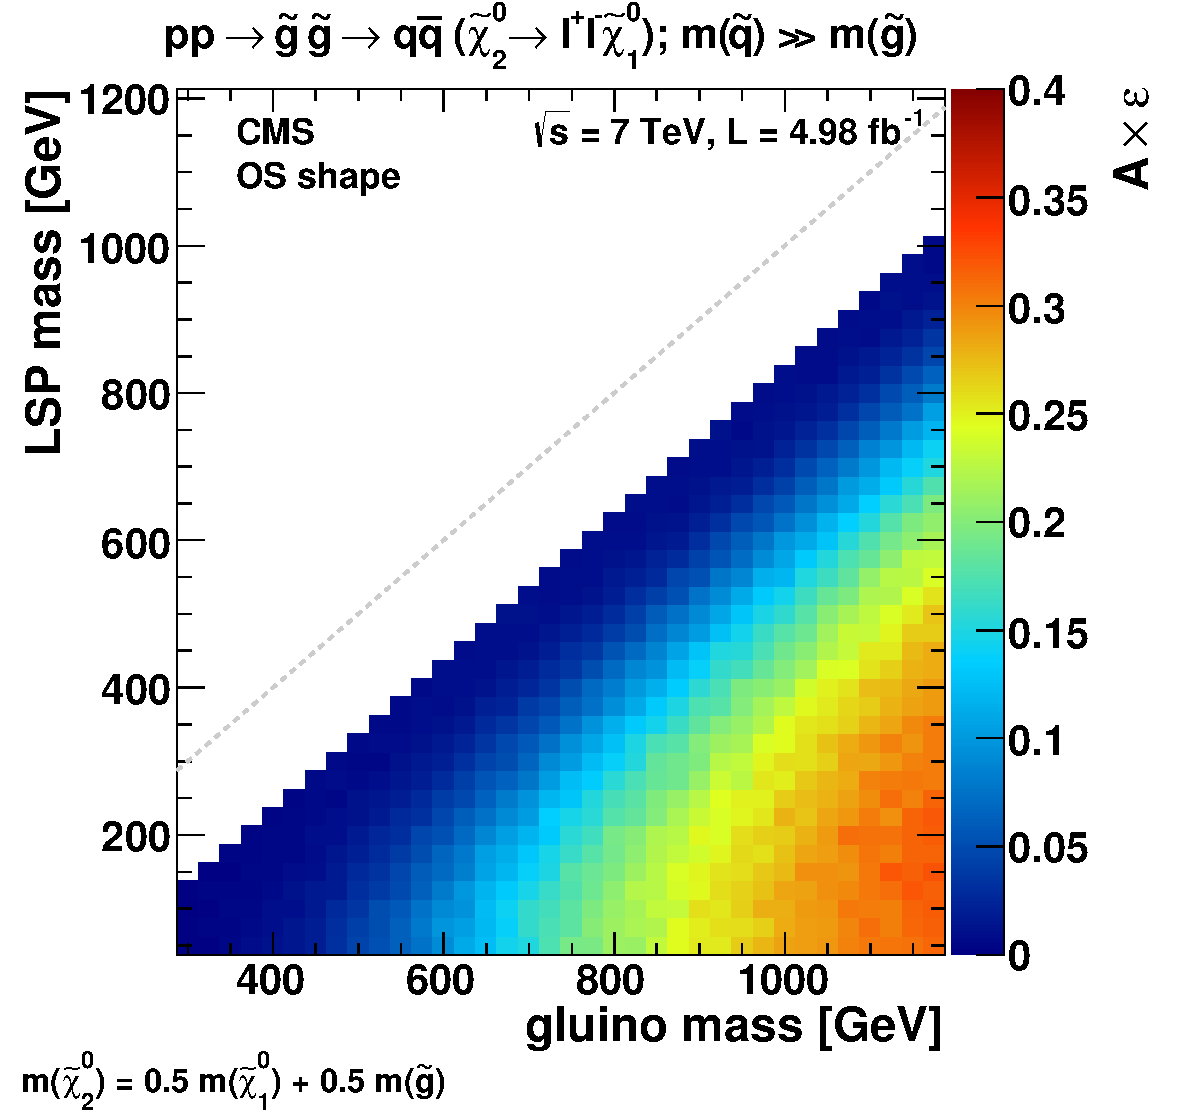
\includegraphics[width=0.5\linewidth]{figures/h_eff_T3lh_OSshape.pdf}} &
\subfigure[\label{fig:smsexampleul}upper limits on production cross
section]
{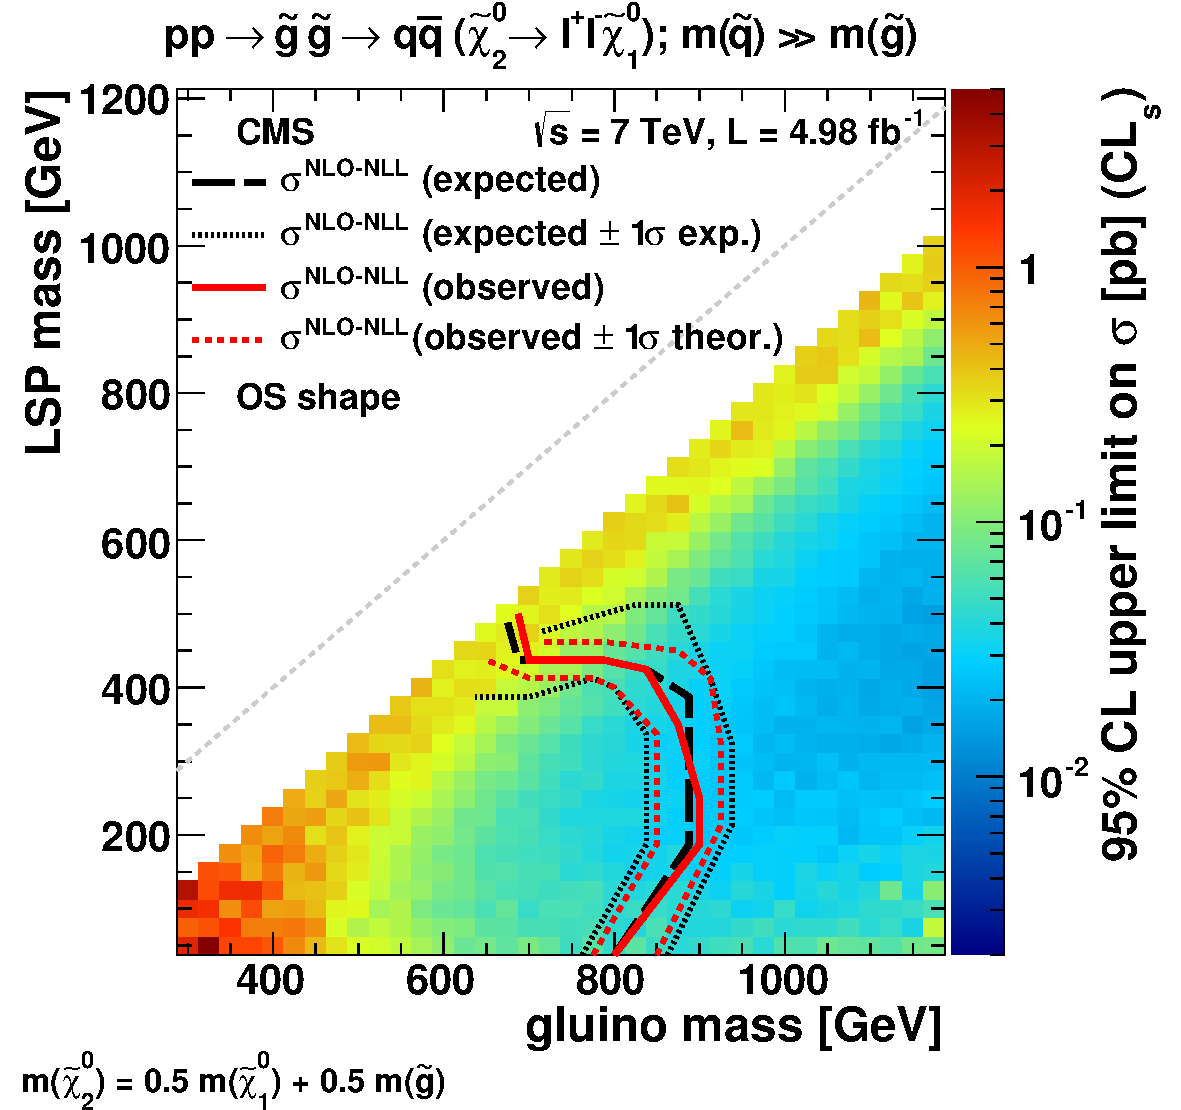
\includegraphics[width=0.5\linewidth]{figures/h_limit_T3lh_OSshape.pdf}}
\\
\end{tabular}
\caption{An example of an SMS result of the CMS collaboration, taken
from~\cite{cms:2013wc}.}
\label{fig:smsexample}
\end{center}
\end{figure}

This document builds upon the 95\% upper limits on \sigmaXBF -- neither the
efficiency plots nor the exclusion lines are of any relevance for this work.
It is however a long-standing wish of the authors to the experimental
collaborations to publish not only the 95\% upper limits, but rather the entire
likelihoods.  This would e.g. allow combinations of LHC results with
uncorrelated non-LHC measurements.  
A combination of several LHC results would still not be feasible because 
the correlations between the SMS results are unknown.
It is an even longer term vision that all ingredients that enter
into the statistical procedure are published also;
in an ideal world a user of the LHC results would be able to produce 
a likelihood for any combination of SMS results published, be they from CMS or
ATLAS.

\subsection{LHC results used}
\label{ssec:lhc}
The SMS results that are currently included in the database are:
\fixme{In the end we will need a clean up and discuss only those results that
we actually used.}
A description of many CMS results used in this document is given in
Ref.~\cite{cms:2013wc}. The ATLAS results are described in
Ref.~\cite{Okawa:2011xg}. 
\fixme{\cite{Okawa:2011xg} only describes hadronic and di-leptonic results, but
I am sure we will use different atlas sms results. Synchronize! Check if there
is an adequate ATLAS legacy paper}

\begin{itemize}
\item {\bf CMS, All-Hadronic:} \AlphaT~\cite{SUS-11-022}, \HsTjets~\cite{SUS-12-011}, \MTtwo~\cite{SUS-12-002} 
\item {\bf CMS, Single-Leptonic:} $\emu$ LS, $\emu$ LP, $\emu$ ANN~\cite{SUS-12-010}
\item {\bf CMS, Inclusive:} razor~\cite{SUS-12-005}, razor+b~\cite{SUS-11-024}
\item {\bf CMS, Di-Leptons:} SS $\emu$~\cite{SUS-11-010}, SS+b~\cite{SUS-11-020}, comb. leptons~\cite{SUS-12-006}, OS $\emu +\ETslash$~\cite{SUS-11-011}, OS \emu edge~\cite{SUS-11-011}, OS \emu ANN~\cite{SUS-11-018}
\item {\bf CMS, Di-Leptons from Z:} \ZMET, JZB~\cite{SUS-11-021}
\item {\bf CMS, Multi-Leptons:} multi leptons~\cite{SUS-11-013}, comb. leptons~\cite{SUS-12-006}
\item {\bf CMS, Stop searches:} razor~\cite{SUS-12-005},
razor+b~\cite{SUS-11-024}, razor+jets~\cite{SUS-12-009},
\AlphaT~\cite{SUS-11-022}, hadronic-\sTop~\cite{SUS-11-030}, leptonic \sTop~\cite{SUS-12-023}, \fixme{dileptonic \sTop, hadronic \sTop at 8 TeV}
\item {\bf ATLAS, Third-generation:} \ATLLepStop~\cite{ATLAS-CONF-2012-166}, \ATLHadStop~\cite{ATLAS-CONF-2013-001}
\item {\bf ...}
\end{itemize}

\fixme{Once theyre out, need to add: alphaT8TeV, mono jets 8 tev, razor mono 8 tev, RA2}



%%%%%%%%%%%%%%%%%%%%%%%%%%%%%%%%%%%%%%%%
\section{Decomposition into simplified model topologies}
%%%%%%%%%%%%%%%%%%%%%%%%%%%%%%%%%%%%%%%%
\subsection{SMS decomposition: The procedure}
\label{ssec:decomp}

Starting point of the SMS decomposition is an SLHA file which contains the
mass spectrum and decay table of a specific MSSM parameter point.
Next, the SLHA file is passed to pythia to generate 10000 events. 
As an output format we chose the LHE file format.
Per event, we then count the SUSY particles, with the SUSY ``mothers'' (i.e.
the first SUSY particles in the decay chains) playing a special role.
Assuming $\chiz$ to always be the LSP  and taking into account conservation of
R-parity, we found the categorization scheme given in
Tab.~\ref{tab:classmothers} to be sufficient. 
Within these categories the events are further categorized based on the 
remaining SUSY particle content. Tabs.~\ref{tab:classgluinos},\ref{tab:classsquarks},\ref{tab:classstops},\ref{tab:classsbottoms},\ref{tab:classweakinos} 
discuss these subcategories. The events' requirements on the particle content is listed, in order for the event to be classified as a specific simplified model.
The requirement on the SUSY mothers and the requirement on the LSPs are not listed.
Fig.~\ref{fig:smsdecomposition} shows an overview of the whole procedure of SMS decomposition.

\begin{table}[h!t]\centering
\begin{tabular}{|c|c|c|}
\hline
Requirement on  & SMS & discussed \\
SUSY mothers  & case  & in Sec. \\
\hline
two gluinos & ``gluinos'' & Sec.~\ref{ssec:gluinocase} \\
two squarks (\first, \second gen) & ``squarks'' & Sec.~\ref{ssec:squarkcase} \\
one gluino, one squark (any generation) & ``associate'' & not discussed \\
two stops & ``stops'' & Sec.~\ref{ssec:thirdcase} \\
two sbottoms & ``sbottoms'' & Sec.~\ref{ssec:thirdcase} \\
two weakinos & ``weakinos'' & Sec.~\ref{ssec:weakinocase} \\
two sleptons & ``sleptons'' & not discussed \\
\hline
\end{tabular}
\caption{Classification of events according to SUSY mothers}
\label{tab:classmothers}
\end{table}

\begin{figure}[h!t]\centering
% \begin{tikzpicture}[anchor=mid,>=latex',line join=bevel,]
\begin{tikzpicture}[>=latex',line join=bevel,]
  \pgfsetlinewidth{1bp}
\begin{small}%
\pgfsetcolor{black}
  % Edge: gg -> T5
  \draw [->] (126.57bp,397.05bp) .. controls (135.39bp,391.92bp) and (149.05bp,384.92bp)  .. (162bp,382bp) .. controls (196.2bp,374.3bp) and (235.83bp,374.32bp)  .. (276.33bp,376.82bp);
  \definecolor{strokecol}{rgb}{0.0,0.0,0.0};
  \pgfsetstrokecolor{strokecol}
  \draw (195bp,393bp) node {qqqqV$^{(*)}$V$^{(*)}$};
  % Edge: tt -> T2tt
  \draw [->] (128.16bp,199.13bp) .. controls (154.04bp,201.76bp) and (219.44bp,208.4bp)  .. (275.35bp,214.08bp);
  \draw (195bp,218bp) node {tt};
  % Edge: ss -> T2
  \draw [->] (128.16bp,320.19bp) .. controls (154.72bp,323.02bp) and (222.91bp,330.29bp)  .. (278.9bp,336.26bp);
  \draw (195bp,339bp) node {qq};
  % Edge: lsp -> nn
  \draw [->] (36.796bp,245.22bp) .. controls (54.879bp,207.07bp) and (90.966bp,130.93bp)  .. (112.28bp,85.962bp);
  % Edge: bb -> T6ttWW
  \draw [->] (128.38bp,265.1bp) .. controls (137.42bp,262.95bp) and (150.43bp,260.18bp)  .. (162bp,259bp) .. controls (192.86bp,255.84bp) and (227.43bp,255.37bp)  .. (265.95bp,255.98bp);
  \draw (195bp,268bp) node {ttWW};
  % Edge: lsp -> gg
  \draw [->] (40.219bp,289.09bp) .. controls (58.037bp,315.53bp) and (88.262bp,360.37bp)  .. (110.67bp,393.61bp);
  % Edge: bb -> T2bb
  \draw [->] (128.44bp,270.46bp) .. controls (137.51bp,272.38bp) and (150.54bp,275.03bp)  .. (162bp,277bp) .. controls (195.61bp,282.79bp) and (233.59bp,288.29bp)  .. (273.26bp,293.71bp);
  \draw (195bp,295bp) node {bb};
  % Edge: nn -> TChiwz
  \draw [->] (143.16bp,78.656bp) .. controls (172.34bp,81.618bp) and (220.39bp,86.497bp)  .. (268.46bp,91.377bp);
  \draw (195bp,96bp) node {WZ};
  % Edge: tt -> T6bbWW
  \draw [->] (123.36bp,188.54bp) .. controls (131.1bp,177.87bp) and (145.25bp,160.99bp)  .. (162bp,153bp) .. controls (190.39bp,139.46bp) and (225.07bp,135.03bp)  .. (264.16bp,134.01bp);
  \draw (195bp,162bp) node {bbWW};
  % Edge: lsp -> ss
  \draw [->] (48.494bp,280.61bp) .. controls (63.718bp,289.14bp) and (83.605bp,300.28bp)  .. (107.01bp,313.4bp);
  % Edge: gg -> T1
  \draw [->] (124.4bp,411.38bp) .. controls (132.67bp,420.18bp) and (146.89bp,433.74bp)  .. (162bp,441bp) .. controls (195.65bp,457.17bp) and (237.5bp,464.63bp)  .. (278.93bp,469.08bp);
  \draw (195bp,470bp) node {qqqq};
  % Edge: lsp -> bb
  \draw [->] (51.834bp,268bp) .. controls (65.489bp,268bp) and (82.071bp,268bp)  .. (105.45bp,268bp);
  % Edge: nn -> TChiN2C1
  \draw [->] (133.23bp,67.857bp) .. controls (141.6bp,64.088bp) and (152.1bp,60.007bp)  .. (162bp,58bp) .. controls (191.37bp,52.042bp) and (224.6bp,50.779bp)  .. (262.48bp,51.452bp);
  \draw (195bp,67bp) node {lll};
  % Edge: lsp -> tt
  \draw [->] (46.196bp,252.46bp) .. controls (62.304bp,240.07bp) and (84.615bp,222.91bp)  .. (107.92bp,204.98bp);
  % Edge: gg -> T3
  \draw [->] (128.16bp,404.3bp) .. controls (151.79bp,407.06bp) and (208.4bp,413.67bp)  .. (263.15bp,420.06bp);
  \draw (195bp,426bp) node {qqqqV$^{(*)}$};
  % Edge: nn -> TChiSlep
  \draw [->] (122.82bp,65.896bp) .. controls (130.25bp,54.068bp) and (144.28bp,34.959bp)  .. (162bp,26bp) .. controls (184.46bp,14.642bp) and (211.16bp,9.6441bp)  .. (245.96bp,7.2855bp);
  \draw (195bp,36.5bp) node {\slep$|$\snu lll};
  % Edge: tt -> T2FVttcc
  \draw [->] (127.11bp,193.37bp) .. controls (136.07bp,189.51bp) and (149.61bp,184.31bp)  .. (162bp,182bp) .. controls (192.05bp,176.41bp) and (226.01bp,175.06bp)  .. (264.3bp,175.39bp);
  \draw (195bp,190bp) node {cc};
  % Node: TChiSlep
\begin{scope}
  \definecolor{strokecol}{rgb}{0.0,0.0,0.0};
  \pgfsetstrokecolor{strokecol}
  \draw (382bp,22bp) -- (246bp,23bp) -- (246bp,0bp) -- (382bp,0bp) -- cycle;
  \draw (314bp,11bp) node {\;\;\;\;\model{TChiSlep*} [Figs.~\ref{fig:TChiChipmSlepSlep},\ref{fig:TChiChipmSnuSlep}] \;\;};
\end{scope}
  % Node: T6ttWW
\begin{scope}
  \definecolor{strokecol}{rgb}{0.0,0.0,0.0};
  \pgfsetstrokecolor{strokecol}
  \draw (362bp,270bp) -- (266bp,270bp) -- (266bp,247bp) -- (362bp,247bp) -- cycle;
  \draw (314bp,258bp) node {\model{T6ttWW} [Fig.~\ref{fig:T6ttWW}]};
\end{scope}
  % Node: TChiwz
\begin{scope}
  \definecolor{strokecol}{rgb}{0.0,0.0,0.0};
  \pgfsetstrokecolor{strokecol}
  \draw (359bp,108bp) -- (269bp,108bp) -- (269bp,85bp) -- (359bp,85bp) -- cycle;
  \draw (314bp,96bp) node {\model{TChiwz} [Fig.~\ref{fig:TChiwz}]};
\end{scope}
  % Node: nn
\begin{scope}
  \definecolor{strokecol}{rgb}{0.0,0.0,0.0};
  \pgfsetstrokecolor{strokecol}
  \definecolor{fillcol}{rgb}{0.9,0.9,0.9};
  \pgfsetfillcolor{fillcol}
  \filldraw [opacity=1.0] (117bp,76bp) ellipse (27bp and 10bp);
  \draw (117bp,76bp) node {weakino};
\end{scope}
  % Node: bb
\begin{scope}
  \definecolor{strokecol}{rgb}{0.0,0.0,0.0};
  \pgfsetstrokecolor{strokecol}
  \definecolor{fillcol}{rgb}{0.9,0.9,0.9};
  \pgfsetfillcolor{fillcol}
  \filldraw [opacity=1.0] (117bp,268bp) ellipse (11bp and 12bp);
  \draw (117bp,268bp) node {$\sb\sb$};
\end{scope}
  % Node: ss
\begin{scope}
  \definecolor{strokecol}{rgb}{0.0,0.0,0.0};
  \pgfsetstrokecolor{strokecol}
  \definecolor{fillcol}{rgb}{0.9,0.9,0.9};
  \pgfsetfillcolor{fillcol}
  \filldraw [opacity=1.0] (117bp,319bp) ellipse (11bp and 11bp);
  \draw (117bp,319bp) node {$\sq\sq$};
\end{scope}
  % Node: tt
\begin{scope}
  \definecolor{strokecol}{rgb}{0.0,0.0,0.0};
  \pgfsetstrokecolor{strokecol}
  \definecolor{fillcol}{rgb}{0.9,0.9,0.9};
  \pgfsetfillcolor{fillcol}
  \filldraw [opacity=1.0] (117bp,198bp) ellipse (11bp and 11bp);
  \draw (117bp,198bp) node {$\st\st$};
\end{scope}
  % Node: T5
\begin{scope}
  \definecolor{strokecol}{rgb}{0.0,0.0,0.0};
  \pgfsetstrokecolor{strokecol}
  \draw (351bp,393bp) -- (277bp,393bp) -- (277bp,370bp) -- (351bp,370bp) -- cycle;
  \draw (314bp,381bp) node {\model{T5*} [Fig.~\ref{fig:T5zz}]};
\end{scope}
  % Node: T2
\begin{scope}
  \definecolor{strokecol}{rgb}{0.0,0.0,0.0};
  \pgfsetstrokecolor{strokecol}
  \draw (349bp,352bp) -- (279bp,352bp) -- (279bp,329bp) -- (349bp,329bp) -- cycle;
  \draw (314bp,340bp) node {\model{T2} [Fig.~\ref{fig:T2}]};
\end{scope}
  % Node: T3
\begin{scope}
  \definecolor{strokecol}{rgb}{0.0,0.0,0.0};
  \pgfsetstrokecolor{strokecol}
  \draw (364bp,438bp) -- (264bp,438bp) -- (264bp,415bp) -- (364bp,415bp) -- cycle;
  \draw (314bp,426bp) node {\, \model{T3*} [Figs.~\ref{fig:T3w},\ref{fig:T3C}]\;\;};
\end{scope}
  % Node: T6bbWW
\begin{scope}
  \definecolor{strokecol}{rgb}{0.0,0.0,0.0};
  \pgfsetstrokecolor{strokecol}
  \draw (363bp,149bp) -- (265bp,149bp) -- (265bp,126bp) -- (363bp,126bp) -- cycle;
  \draw (314bp,137bp) node {\model{T6bbWW} [Fig.~\ref{fig:T6bbWW}]};
\end{scope}
  % Node: T1
\begin{scope}
  \definecolor{strokecol}{rgb}{0.0,0.0,0.0};
  \pgfsetstrokecolor{strokecol}
  \draw (349bp,483bp) -- (279bp,483bp) -- (279bp,460bp) -- (349bp,460bp) -- cycle;
  \draw (314bp,471bp) node {\model{T1} [Fig.~\ref{fig:T1}]};
\end{scope}
  % Node: gg
\begin{scope}
  \definecolor{strokecol}{rgb}{0.0,0.0,0.0};
  \pgfsetstrokecolor{strokecol}
  \definecolor{fillcol}{rgb}{0.9,0.9,0.9};
  \pgfsetfillcolor{fillcol}
  \filldraw [opacity=1.0] (117bp,403bp) ellipse (11bp and 11bp);
  \draw (117bp,403bp) node {$\gl\gl$};
\end{scope}
  % Node: T2FVttcc
\begin{scope}
  \definecolor{strokecol}{rgb}{0.0,0.0,0.0};
  \pgfsetstrokecolor{strokecol}
  \draw (363bp,190bp) -- (265bp,190bp) -- (265bp,167bp) -- (363bp,167bp) -- cycle;
  \draw (314bp,178bp) node {\model{T2FVttcc} [Fig.~\ref{fig:T2FVttcc}]};
\end{scope}
  % Node: lsp
\begin{scope}
  \definecolor{strokecol}{rgb}{0.0,0.0,0.0};
  \pgfsetstrokecolor{strokecol}
  \definecolor{fillcol}{rgb}{0.8,0.8,0.8};
  \pgfsetfillcolor{fillcol}
  \filldraw [opacity=1.0] (26bp,268bp) ellipse (25bp and 26bp);
  \draw (26bp,268bp) node {$\chiz$ is LSP};
\end{scope}
  % Node: TChiN2C1
\begin{scope}
  \definecolor{strokecol}{rgb}{0.0,0.0,0.0};
  \pgfsetstrokecolor{strokecol}
  \draw (365bp,67bp) -- (263bp,67bp) -- (263bp,44bp) -- (365bp,44bp) -- cycle;
  \draw (314bp,55bp) node {\model{TChiN2C1} [Fig.~\ref{fig:TChiN2C1}]};
\end{scope}
  % Node: T2tt
\begin{scope}
  \definecolor{strokecol}{rgb}{0.0,0.0,0.0};
  \pgfsetstrokecolor{strokecol}
  \draw (352bp,230bp) -- (276bp,230bp) -- (276bp,207bp) -- (352bp,207bp) -- cycle;
  \draw (314bp,218bp) node {\model{T2tt} [Fig.~\ref{fig:T2tt}]};
\end{scope}
  % Node: T2bb
\begin{scope}
  \definecolor{strokecol}{rgb}{0.0,0.0,0.0};
  \pgfsetstrokecolor{strokecol}
  \draw (354bp,311bp) -- (274bp,311bp) -- (274bp,288bp) -- (354bp,288bp) -- cycle;
  \draw (314bp,299bp) node {\model{T2bb} [Fig.~\ref{fig:T2bb}]};
\end{scope}
\end{small}%
\end{tikzpicture}

\label{fig:smsdecomposition}
\caption{Schematics of the whole SMS decomposition procedure}
\end{figure}


Note, that SMS decomposition can also be performed on the SLHA files directly.
In this note, we chose an SMS decomposition procedure based on LHE files; for a
first document attempt at SMS decomposition this seemed to be the safer
approach. For later studies we envisage employing a SLHA-based SMS decomposition,
in addition to the LHE-based approach.

\FloatBarrier


%%%%%%%%%%%%%%%%%%%%%%%%%%%%%%%%%%%%%%%%
\section{Parameter scan}
%%%%%%%%%%%%%%%%%%%%%%%%%%%%%%%%%%%%%%%%

For the sake of definiteness we scan over a 7 parameter semi-constrained version of the MSSM 
with parameters defined at the GUT scale. 
Concretely, we take a universal gaugino mass parameter $M_{1/2}$,  as well as common scalar mass parameters 
for first and second generation sfermions ($M_{0,1}$) and third generation sfermions ($M_{0,3}$) at $\mgut$.  
We also assume a common trilinear coupling $A_0\equiv A_t=A_b=A_\tau$ at $\mgut$. 
Regarding the Higgs sector,  we trade $M_{H_u}^2$ and $M_{H_d}^2$ at $\mgut$ against 
$\mu$ and $m_A$ at the SUSY scale. Finally, we need the ratio of the two Higgs VEVs, $\tan\beta=v_2/v_1$, 
which we define at the weak scale. 
The scan ranges are given in Table~\ref{tab:scan}.

\begin{table}[t]\centering
\begin{tabular}{|c|c|c|c|c|c|c|c|}
  \hline
  $M_{1/2}$ & $M_{0,1}$ & $M_{0,3}$ & $A_0$ & $m_A$ & $\mu$ & $\tan\beta$ \\ 
  \hline
  0.1\,--\,1 & 0\,--\,3 & 0\,--\,1 & $-3$\,--\,3 & 0.1\,--\,2 & 0.1\,--\,1 & 2\,--\,50 \\
  \hline
\end{tabular}
\caption{Scan ranges used in this study. Dimensionful quantities are in TeV units.}
\label{tab:scan}
\end{table}

\marginpar{\bf add versions and refs}
We use SOFTSUSY for the computation of the masses and mixings,  SUPERISO for flavor observables, 
micrOMEGAs for dark matter observables and particle decay tables, and HDECAY for computing Higgs decays.
For the SM input values, we use $m_t=....$, $m_b(m_b)=4.19$~GeV, and $\alpha_s(M_Z)=0.1187$ ????  
We require a neutralino LSP.  
The constraints imposed are listed in Table~\ref{tab:constraints}.

\begin{table}[t]\centering
\begin{tabular}{|c|c|c|c|c|}
\hline
  \bf Observable  & \bf Experimental result   & \bf TH uncertainty & \bf Constraint imposed \\
\hline
 BR$(b \rightarrow s\gamma) $ & $(3.55 \pm 0.23 \pm 0.09)\times 10^{-4}$ \cite{Amhis:2012bh} & $0.24 \times 10^{-4}$ & $[2.86,\,4.24] \times 10^{-4}$  \\
\hline
BR$(B_s \rightarrow \mu^+ \mu^-)$ & $3.2^{+1.5}_{-1.2} \times 10^{-9}$ \cite{lhcb:2012ct} & 10\% & $[0.7,\,6.3] \times 10^{-9}$\\
\hline
$\Delta a_\mu$ & $(26.1 \pm 8.0)\times 10^{-10}$ \cite{Hagiwara:2011af} & $10\times 10^{-10}$ & $[-0.5,\,51.7] \times 10^{-10}$ \\
\hline
$\Omega h^2$ & $0.1123\pm 0.0055$~\cite{} & 10\% & $<0.136$ \\
\hline
$m_h$ & $125.2\pm 0.3\pm 0.6$ GeV (ATLAS) & 3~GeV \cite{xxx} & $125.5\pm 3$~GeV \\
              & $125.8\pm 0.4\pm 0.4$ GeV (CMS)\phantom{00} & &  \\
\hline
 sparticle masses & LEP  & --- & (micrOMEGAs) \\
\hline
\end{tabular}
\caption{Constraints used to define the valid parameter space before applying the SMS limits.}
\label{tab:constraints}
\end{table}



%%%%%%%%%%%%%%%%%%%%%%%%%%%%%%%%%%%%%%%%
\section{Results}
%%%%%%%%%%%%%%%%%%%%%%%%%%%%%%%%%%%%%%%%


%%%%%%%%%%%%%%%%%%%%%%%%%%%%%%%%%%%%%%%%
\section{Conclusions}
%%%%%%%%%%%%%%%%%%%%%%%%%%%%%%%%%%%%%%%%


\clearpage
%%%%%%%%%%%%%%%%%%%%%%%%%%%%%%%%%%%%%%%%
\section*{Acknowledgements} 
%%%%%%%%%%%%%%%%%%%%%%%%%%%%%%%%%%%%%%%%

This work was supported in part by the by the French 
ANR project {\sc DMAstroLHC}. %BLAN12-???.

\begin{appendix}
\FloatBarrier


\section{Appendix: LHC Results and SMS Topologies}

In Table~\ref{tab:LHCresults} we list the LHC experimental results used in this document and the
corresponding SMS topologies or sets of topologies constrained by each result\fixme{Fix analysis labels and graphs (fix dashed/solid lines). Add more information? Add references. Better looking table.}.
\begin{longtable}{|c|c|} 
   \hline 
  Analysis & SMS Topology \\ 
   \hline 
\multirow{1}{*}{ATLAS-CONF-2013-036 } &  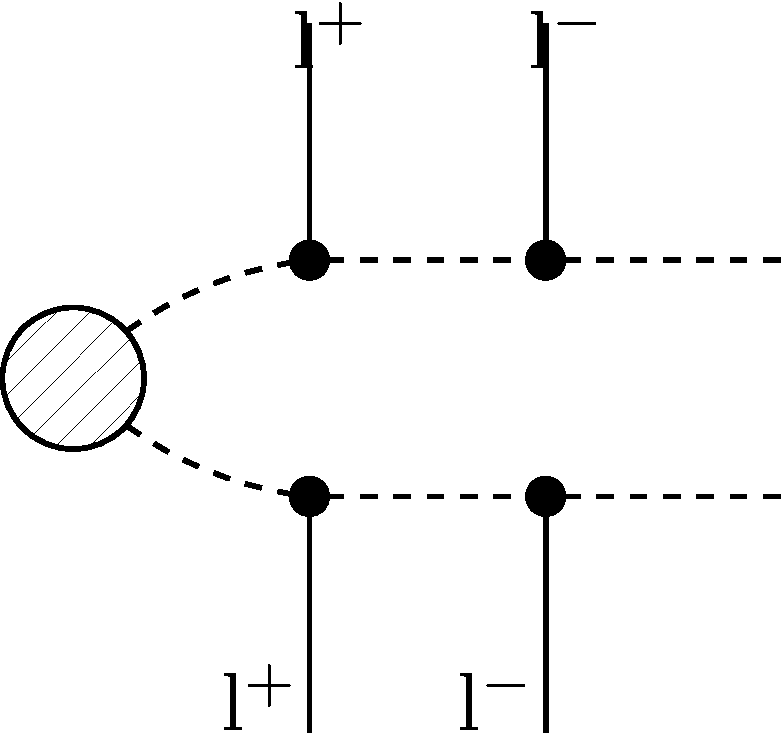
\includegraphics[width=0.15\linewidth]{figures/ATLAS_CONF_2013_036:TChiChiSlepSlep_TChiChiSlepSlep_1_.pdf}\spacer+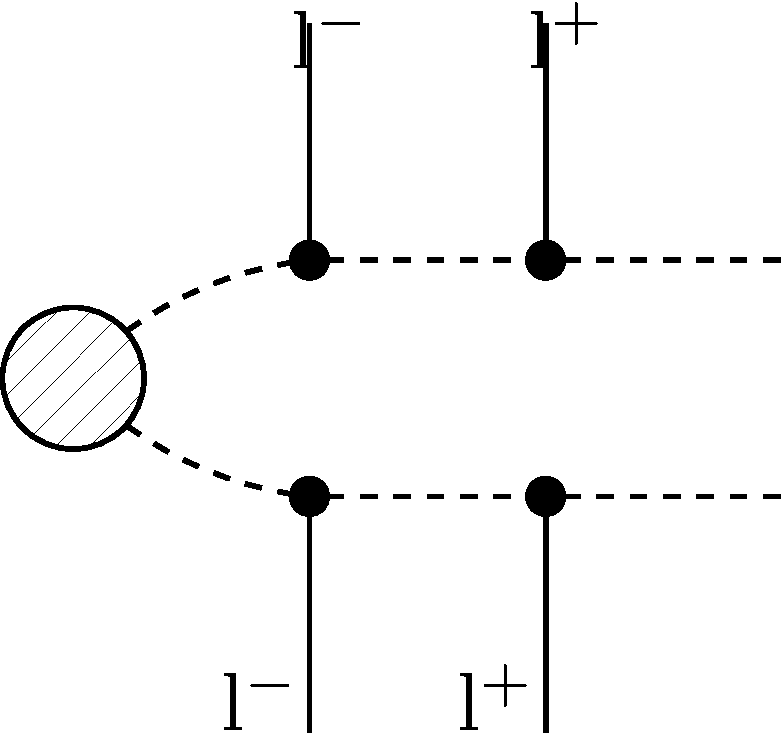
\includegraphics[width=0.15\linewidth]{figures/ATLAS_CONF_2013_036:TChiChiSlepSlep_TChiChiSlepSlep_2_.pdf}\spacer+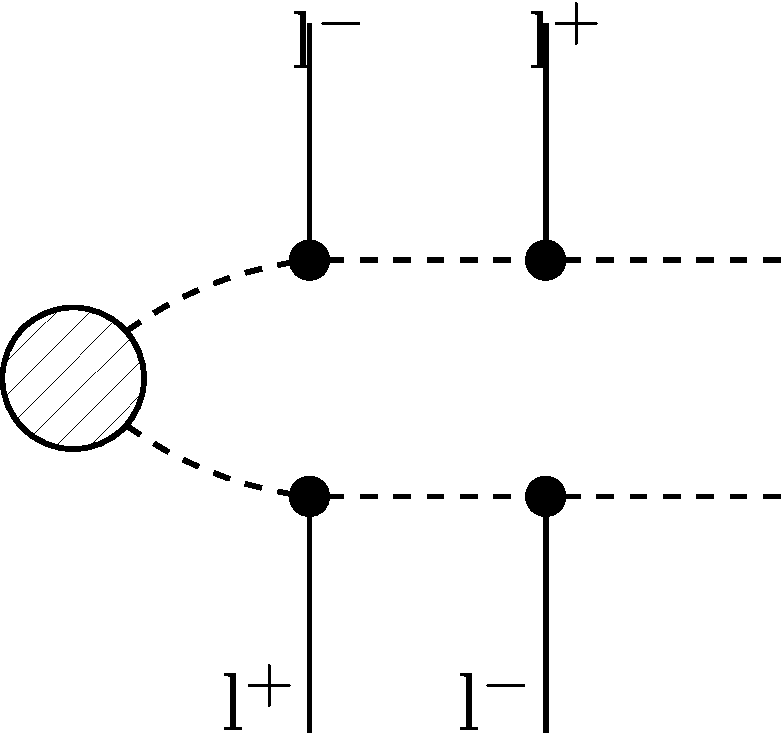
\includegraphics[width=0.15\linewidth]{figures/ATLAS_CONF_2013_036:TChiChiSlepSlep_TChiChiSlepSlep_3_.pdf}\spacer \\  \hline 
\multirow{2}{*}{ATLAS-CONF-2013-037 } &  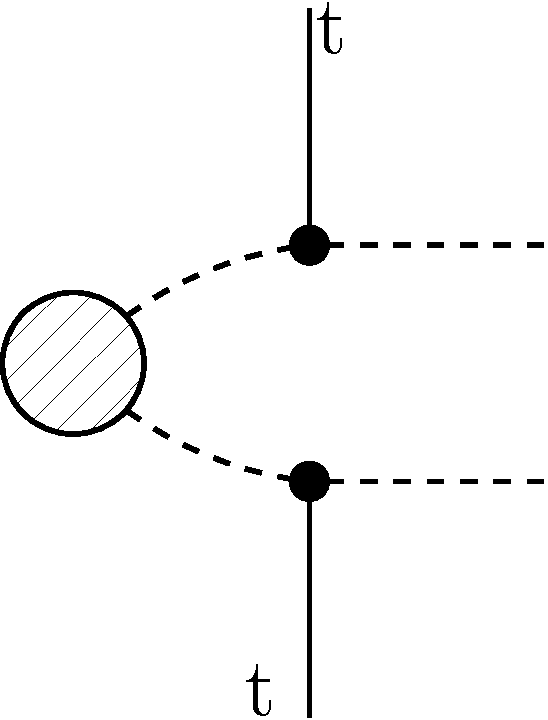
\includegraphics[width=0.15\linewidth]{figures/ATLAS_CONF_2013_037:T2tt_T2tt_1_.pdf}\spacer \\ 
 &  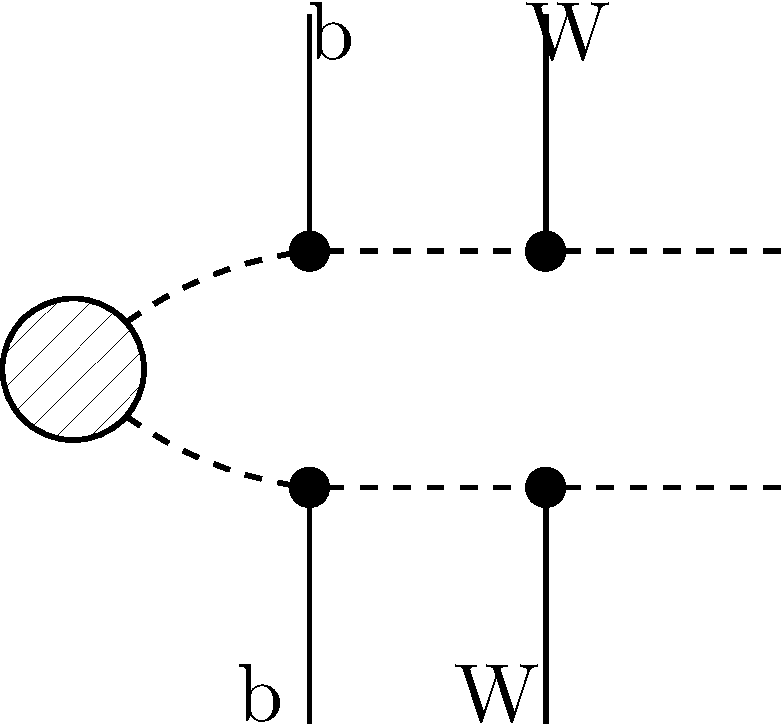
\includegraphics[width=0.15\linewidth]{figures/ATLAS_CONF_2013_037:T6bbWW_T6bbWW_1_.pdf}\spacer \\  \hline 
\multirow{1}{*}{ATLAS-CONF-2013-024 } &  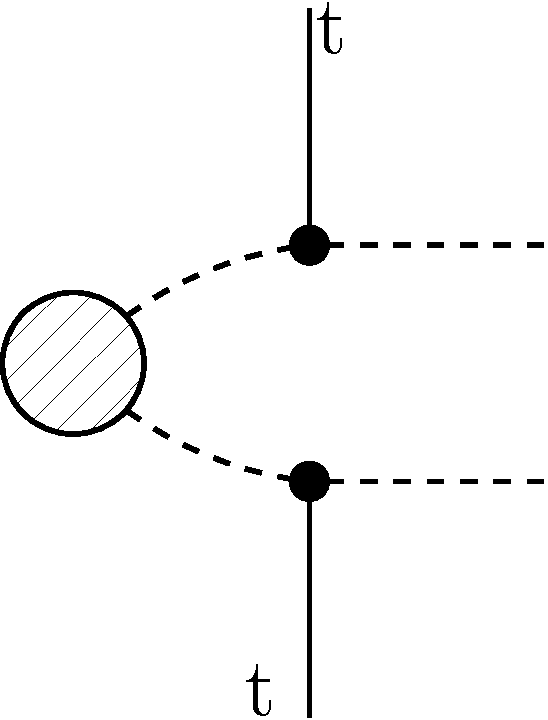
\includegraphics[width=0.15\linewidth]{figures/ATLAS_CONF_2013_024:T2tt_T2tt_1_.pdf}\spacer \\  \hline 
\multirow{1}{*}{MultiLepton8TeV } &  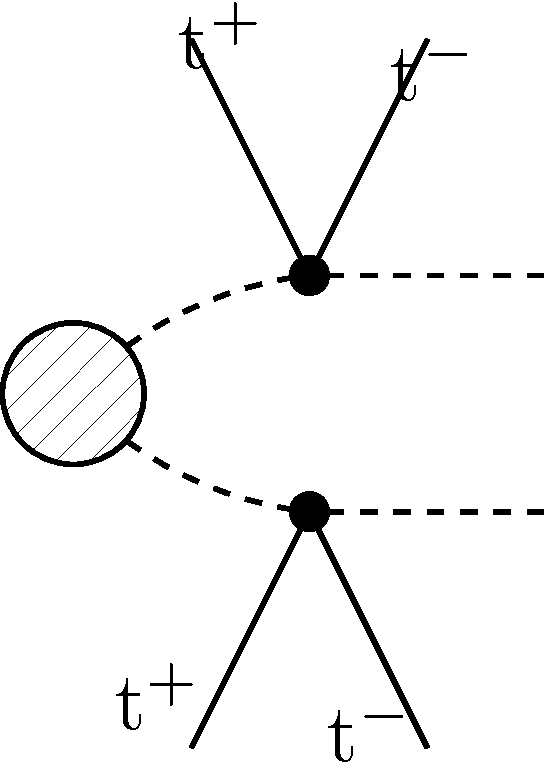
\includegraphics[width=0.15\linewidth]{figures/MultiLepton8TeV:T1tttt_T1tttt_1_.pdf}\spacer \\  \hline 
\multirow{2}{*}{LeptonicStop8TeV } &  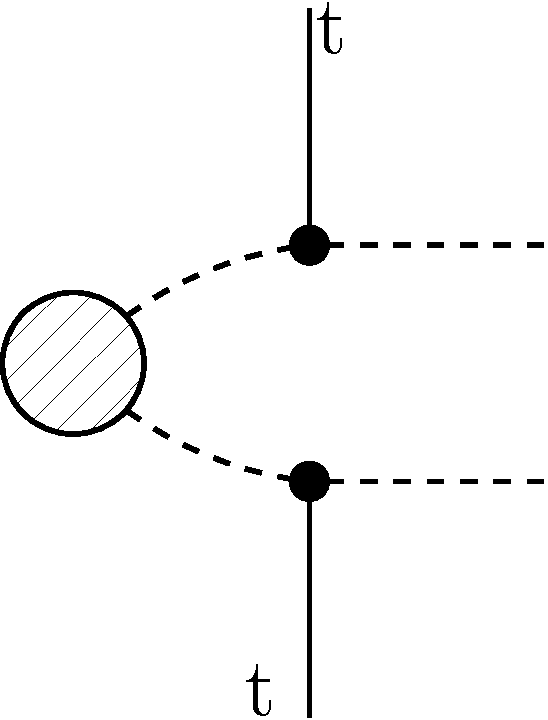
\includegraphics[width=0.15\linewidth]{figures/LeptonicStop8TeV:T2tt_T2tt_1_.pdf}\spacer \\ 
 &  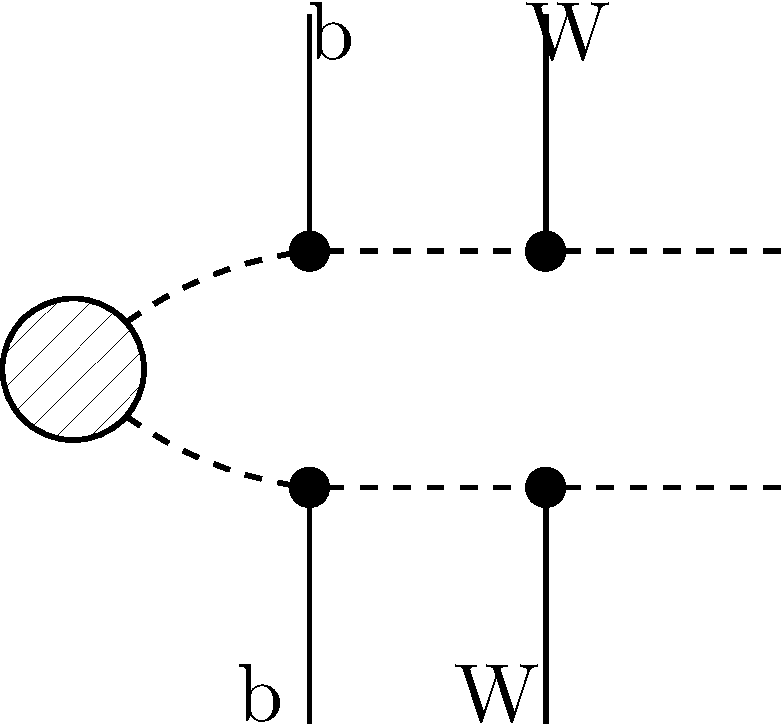
\includegraphics[width=0.15\linewidth]{figures/LeptonicStop8TeV:T6bbWW_T6bbWW_1_.pdf}\spacer \\  \hline 
\multirow{1}{*}{RA4LS8TeV } &  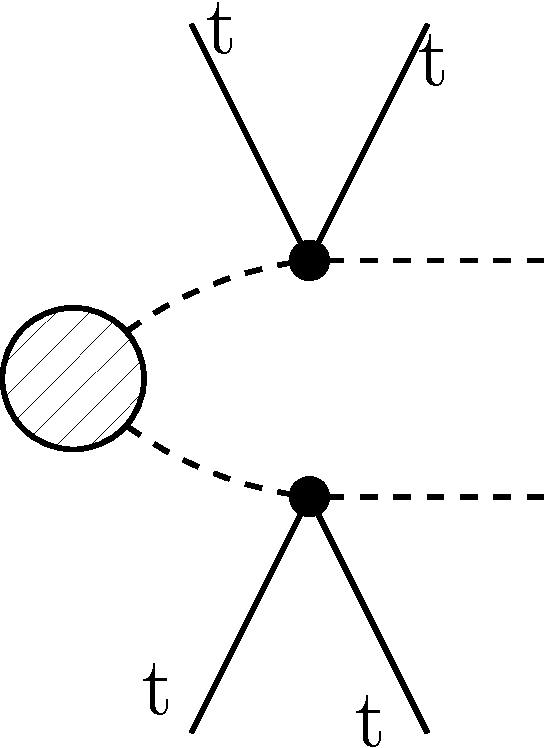
\includegraphics[width=0.15\linewidth]{figures/RA4LS8TeV:T1tttt_T1tttt_1_.pdf}\spacer \\  \hline 
\multirow{2}{*}{ATLAS-CONF-2013-035 } &  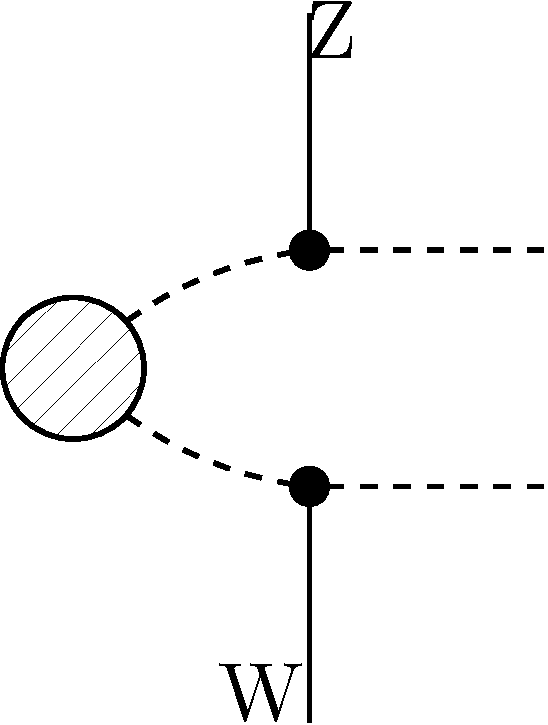
\includegraphics[width=0.15\linewidth]{figures/ATLAS_CONF_2013_035:TChiWZ_TChiWZ_1_.pdf}\spacer \\ 
 &  2.*(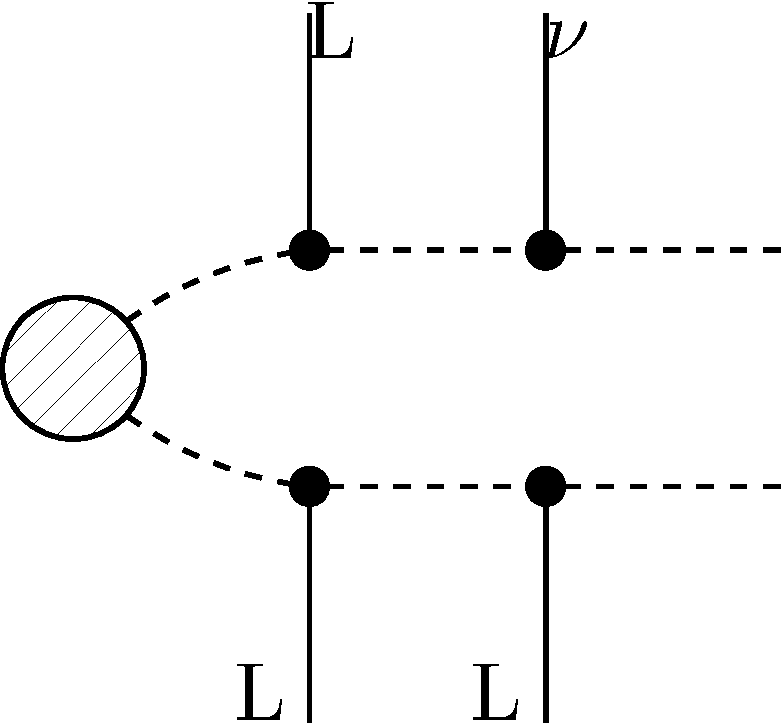
\includegraphics[width=0.15\linewidth]{figures/ATLAS_CONF_2013_035:TChiChipmSlepL_TChiChipmSlepL_1_.pdf}\spacer+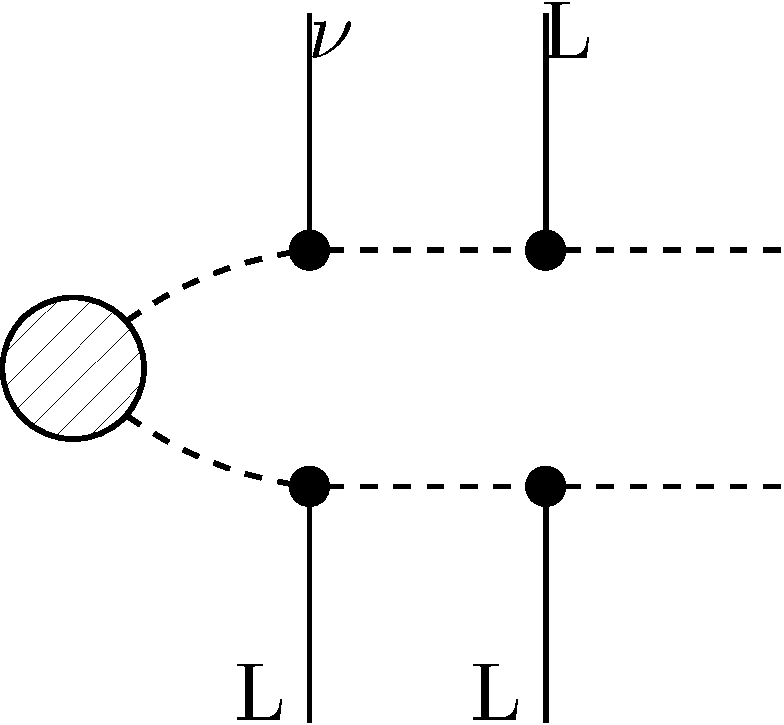
\includegraphics[width=0.15\linewidth]{figures/ATLAS_CONF_2013_035:TChiChipmSlepL_TChiChipmSlepL_2_.pdf}\spacer) \\  \hline 
\multirow{2}{*}{ATLAS-CONF-2012-166 } &  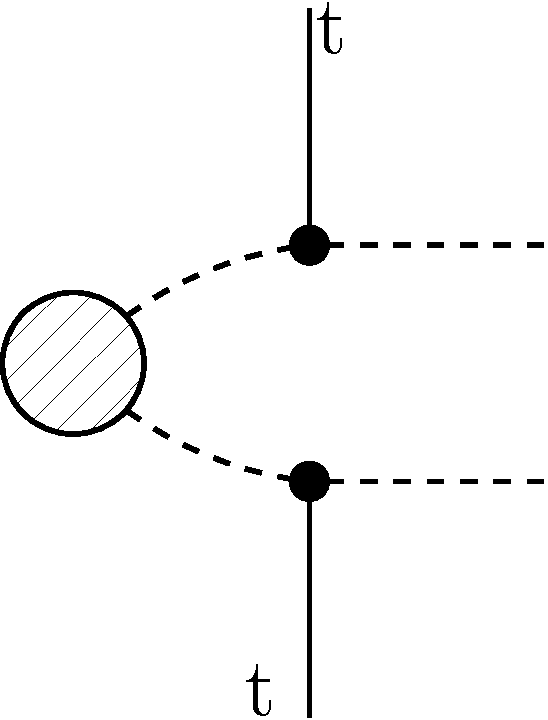
\includegraphics[width=0.15\linewidth]{figures/ATLAS_CONF_2012_166:T2tt_T2tt_1_.pdf}\spacer \\ 
 &  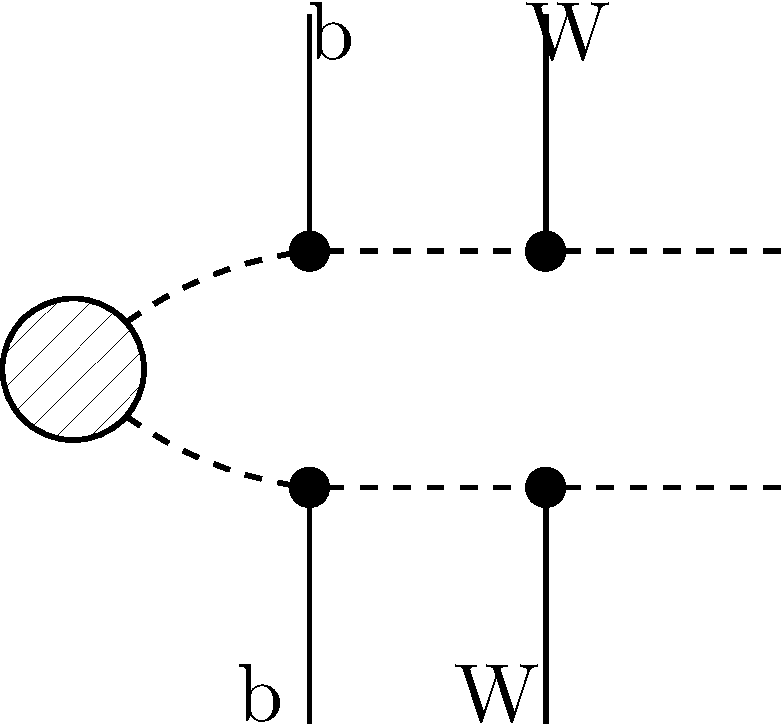
\includegraphics[width=0.15\linewidth]{figures/ATLAS_CONF_2012_166:T6bbWW_T6bbWW_1_.pdf}\spacer \\  \hline 
\multirow{1}{*}{ATLAS-CONF-2013-025 } &  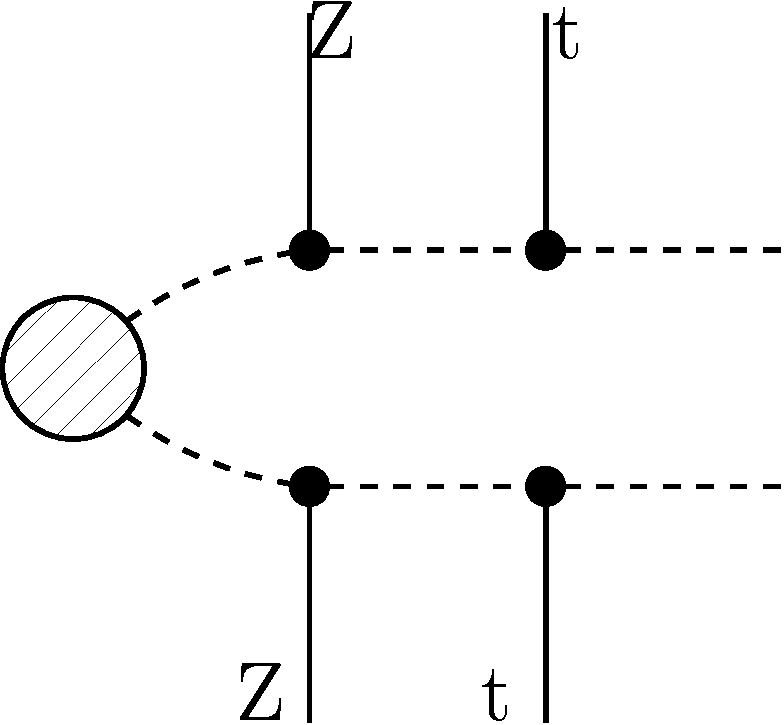
\includegraphics[width=0.15\linewidth]{figures/ATLAS_CONF_2013_025:T6ttZZ_T6ttZZ_1_.pdf}\spacer \\  \hline 
\multirow{6}{*}{alphaT } &  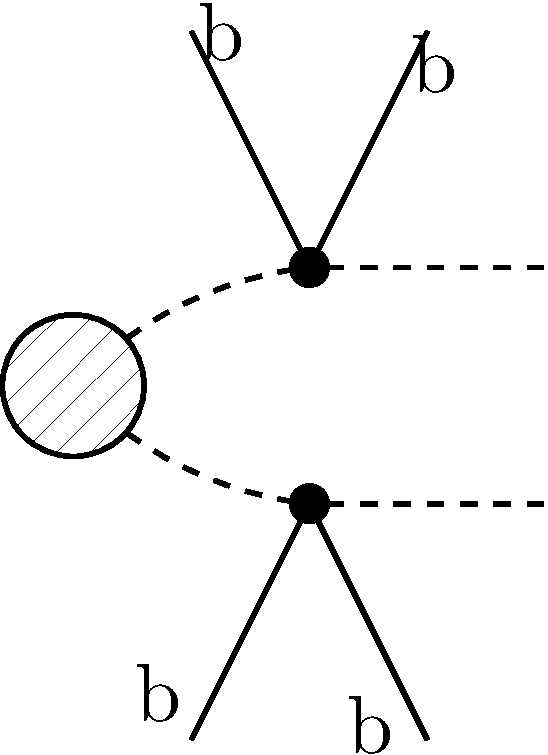
\includegraphics[width=0.15\linewidth]{figures/alphaT:T1bbbb_T1bbbb_1_.pdf}\spacer \\ 
 &  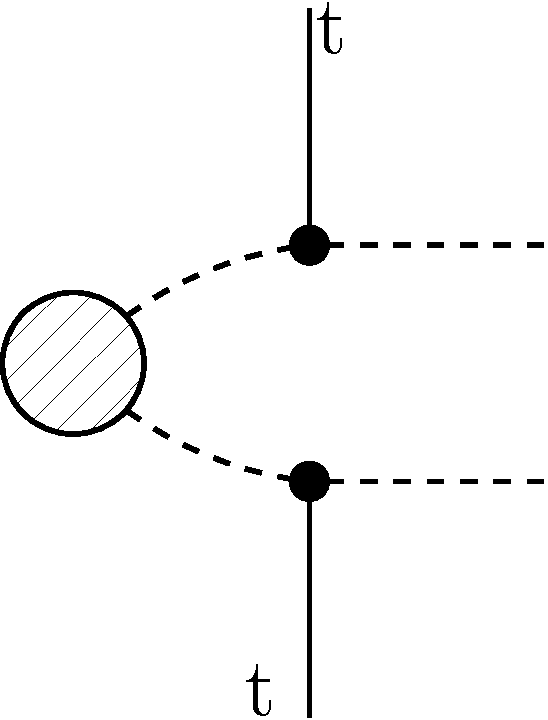
\includegraphics[width=0.15\linewidth]{figures/alphaT:T2tt_T2tt_1_.pdf}\spacer \\ 
 &  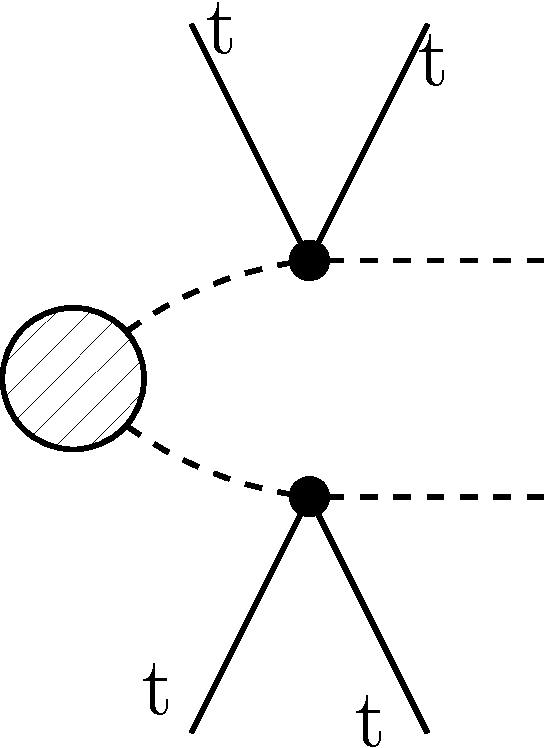
\includegraphics[width=0.15\linewidth]{figures/alphaT:T1tttt_T1tttt_1_.pdf}\spacer \\ 
 &  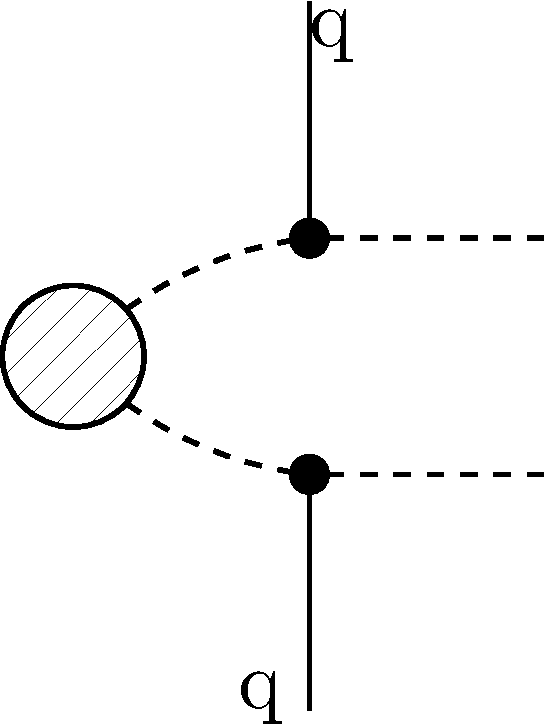
\includegraphics[width=0.15\linewidth]{figures/alphaT:T2_T2_1_.pdf}\spacer \\ 
 &  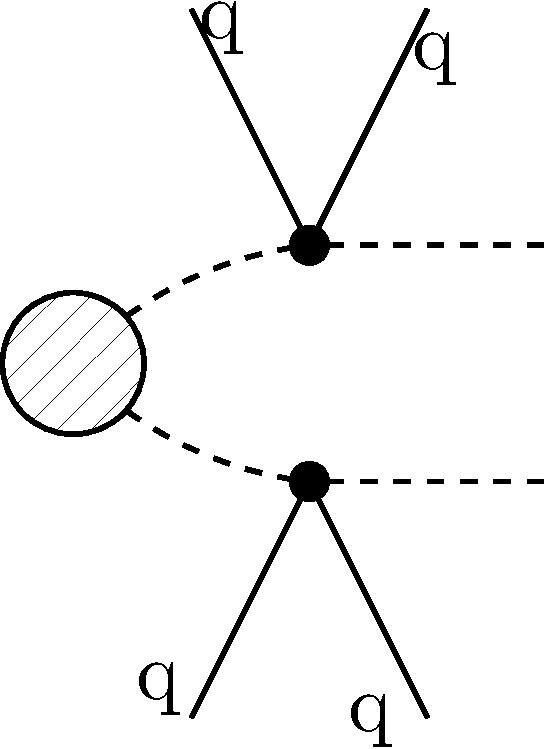
\includegraphics[width=0.15\linewidth]{figures/alphaT:T1_T1_1_.pdf}\spacer \\ 
 &  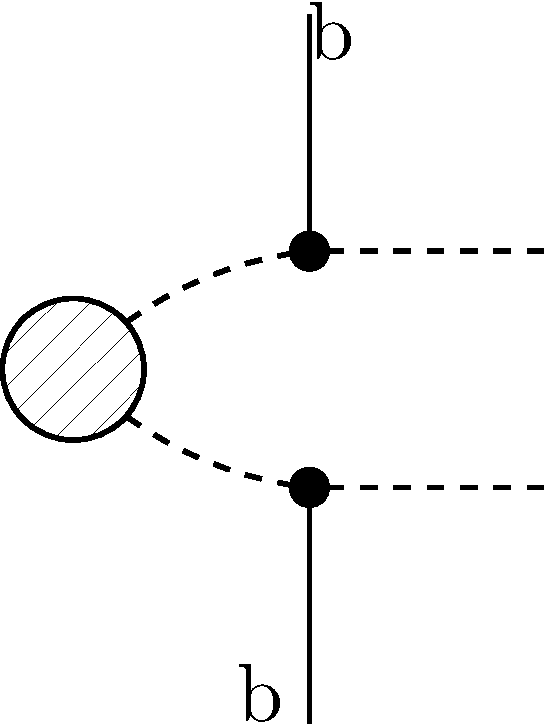
\includegraphics[width=0.15\linewidth]{figures/alphaT:T2bb_T2bb_1_.pdf}\spacer \\  \hline 
\multirow{1}{*}{ATLAS-CONF-2013-001 } &  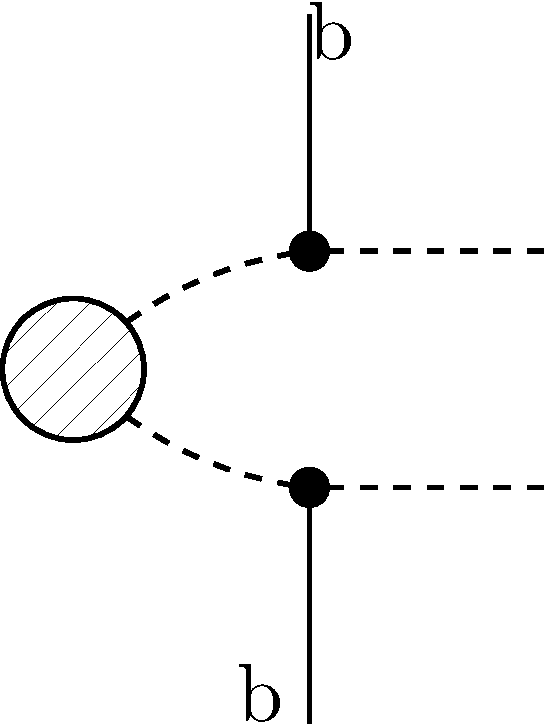
\includegraphics[width=0.15\linewidth]{figures/ATLAS_CONF_2013_001:T2bb_T2bb_1_.pdf}\spacer \\  \hline 
\multirow{5}{*}{ATLAS-CONF-2013-007 } &  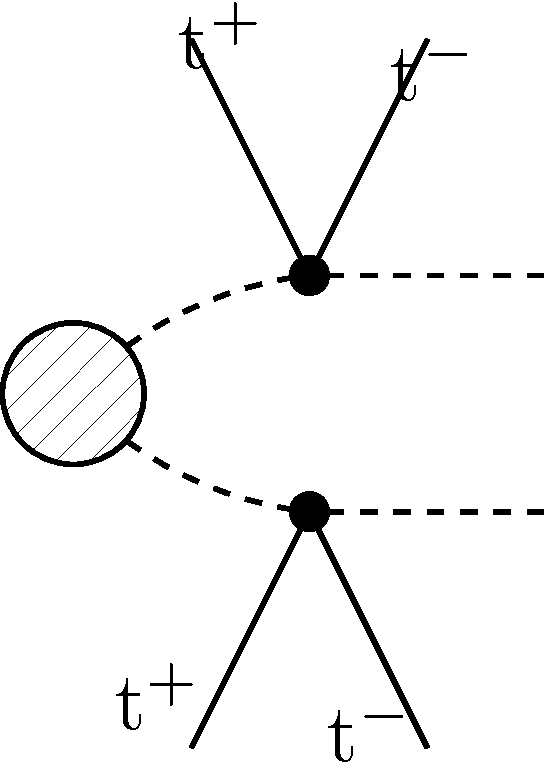
\includegraphics[width=0.15\linewidth]{figures/ATLAS_CONF_2013_007:T1tttt_T1tttt_1_.pdf}\spacer \\ 
 &  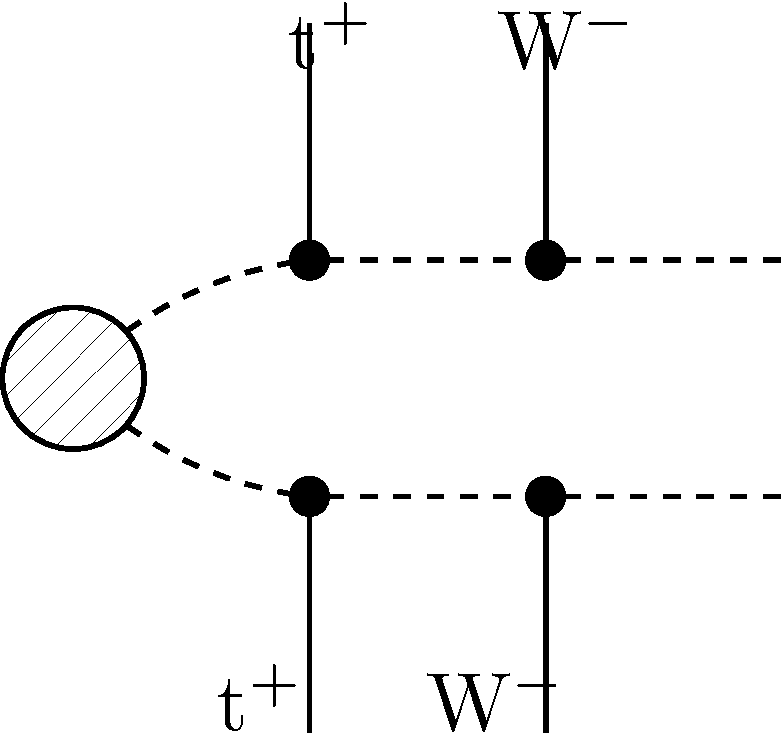
\includegraphics[width=0.15\linewidth]{figures/ATLAS_CONF_2013_007:T6ttWW_T6ttWW_1_.pdf}\spacer+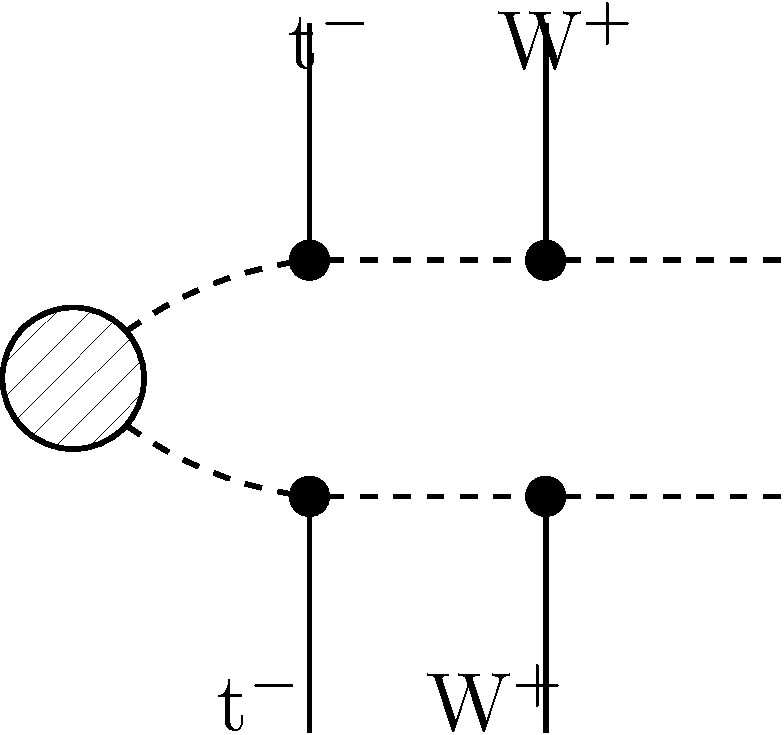
\includegraphics[width=0.15\linewidth]{figures/ATLAS_CONF_2013_007:T6ttWW_T6ttWW_2_.pdf}\spacer+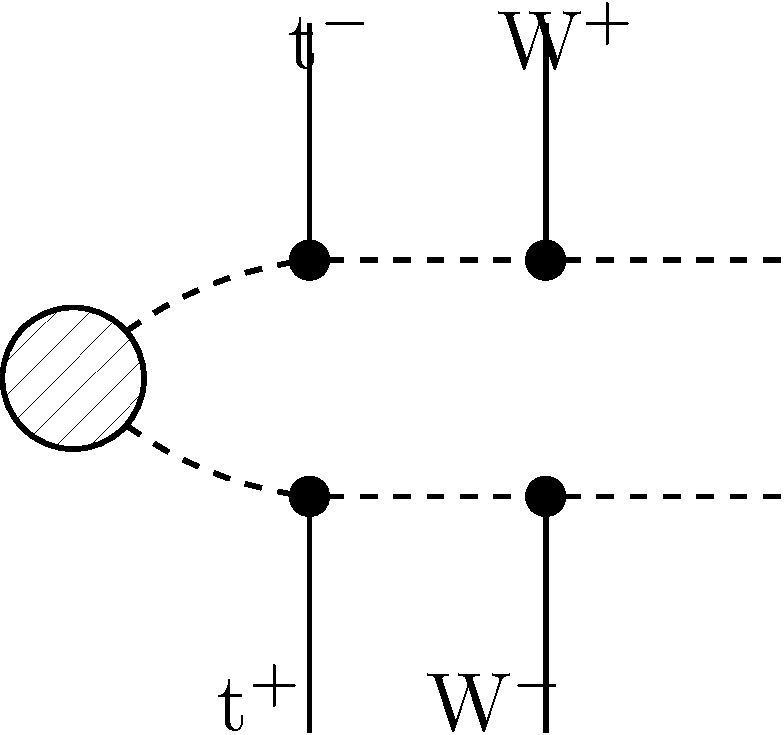
\includegraphics[width=0.15\linewidth]{figures/ATLAS_CONF_2013_007:T6ttWW_T6ttWW_3_.pdf}\spacer \\ 
 &  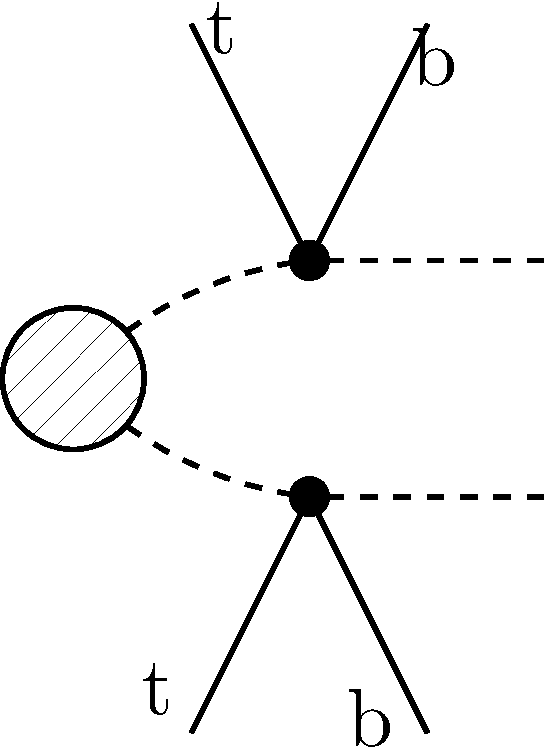
\includegraphics[width=0.15\linewidth]{figures/ATLAS_CONF_2013_007:T1tbtb_T1tbtb_1_.pdf}\spacer \\ 
 &  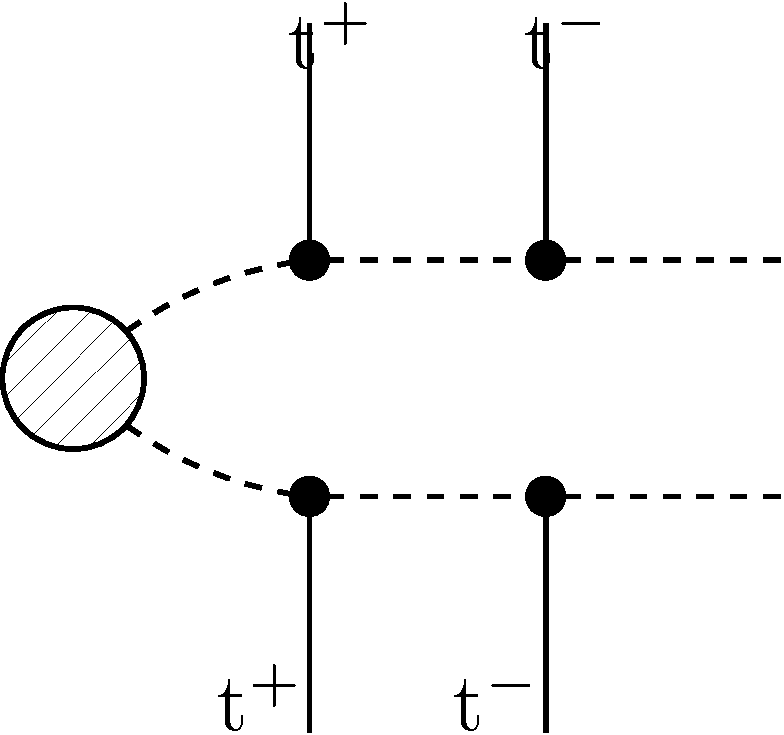
\includegraphics[width=0.15\linewidth]{figures/ATLAS_CONF_2013_007:T5tttt_T5tttt_1_.pdf}\spacer+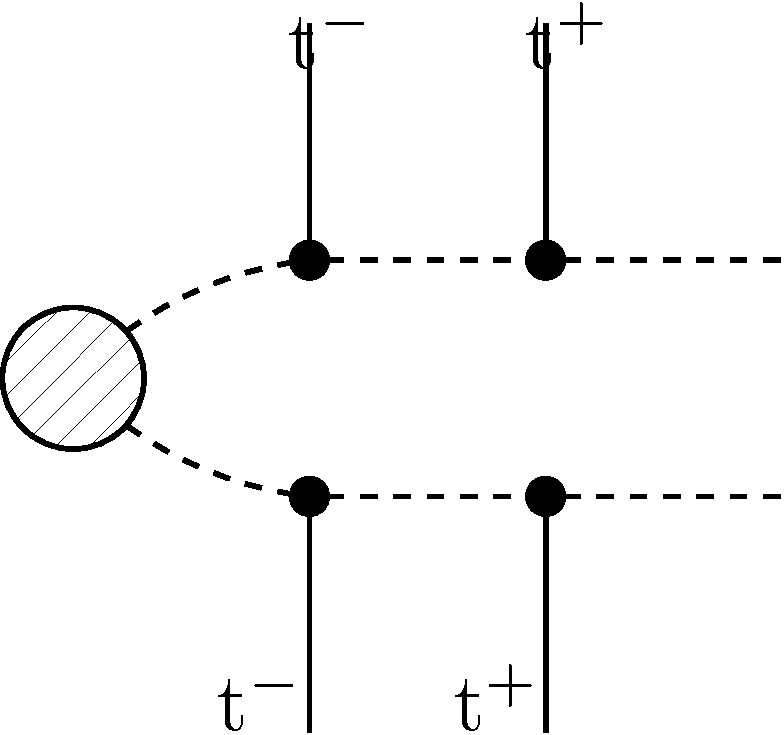
\includegraphics[width=0.15\linewidth]{figures/ATLAS_CONF_2013_007:T5tttt_T5tttt_2_.pdf}\spacer+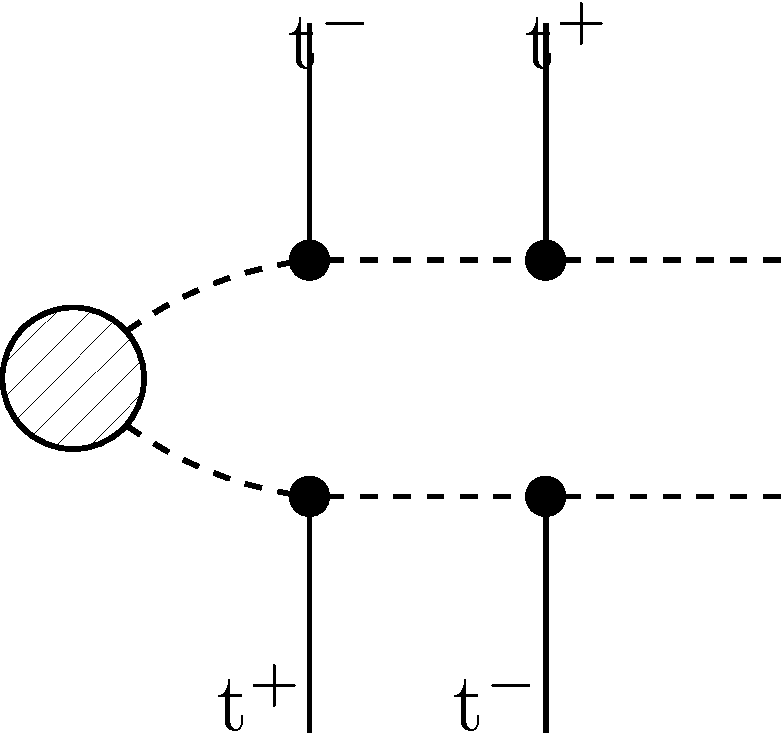
\includegraphics[width=0.15\linewidth]{figures/ATLAS_CONF_2013_007:T5tttt_T5tttt_3_.pdf}\spacer \\ 
 &  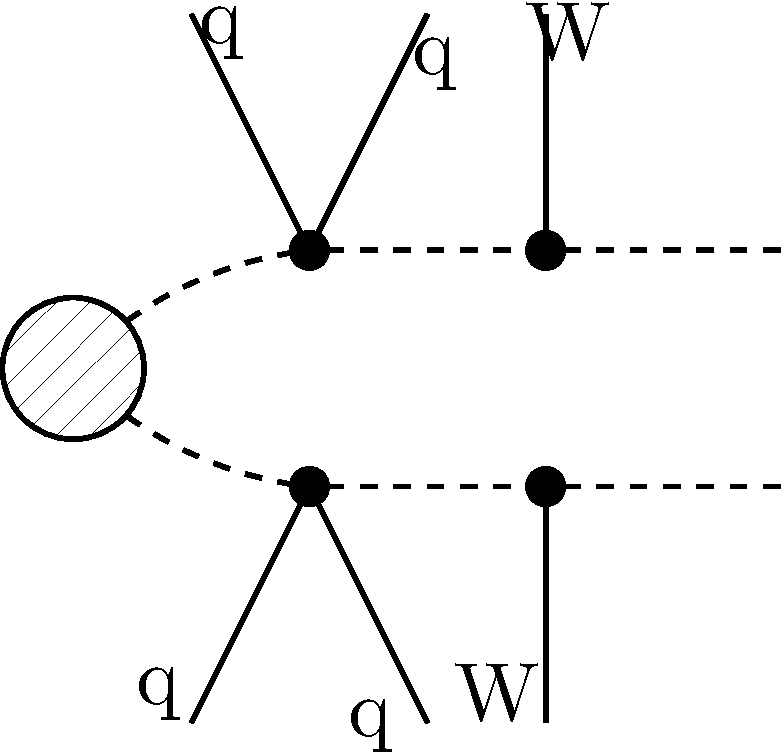
\includegraphics[width=0.15\linewidth]{figures/ATLAS_CONF_2013_007:T5WW_T5WW_1_.pdf}\spacer \\  \hline 
\multirow{2}{*}{ATLAS-CONF-2013-028 } &  2.*(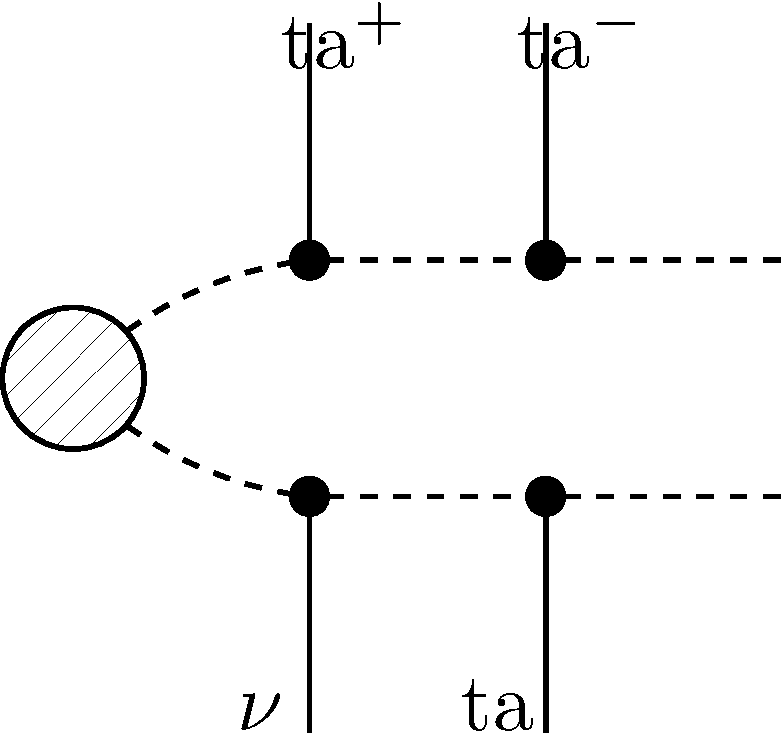
\includegraphics[width=0.15\linewidth]{figures/ATLAS_CONF_2013_028:TChiChipmStauL_TChiChipmStauL_1_.pdf}\spacer+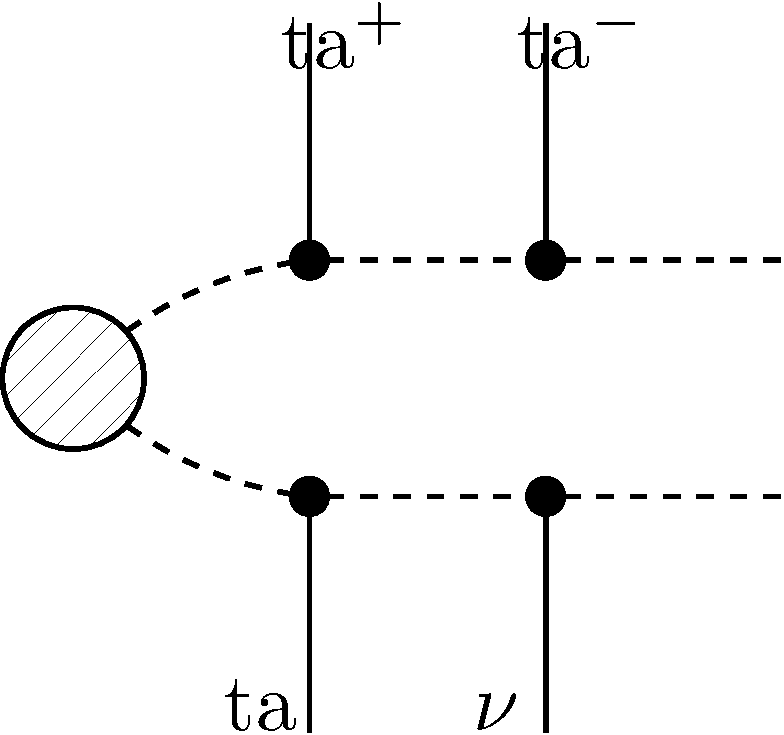
\includegraphics[width=0.15\linewidth]{figures/ATLAS_CONF_2013_028:TChiChipmStauL_TChiChipmStauL_2_.pdf}\spacer+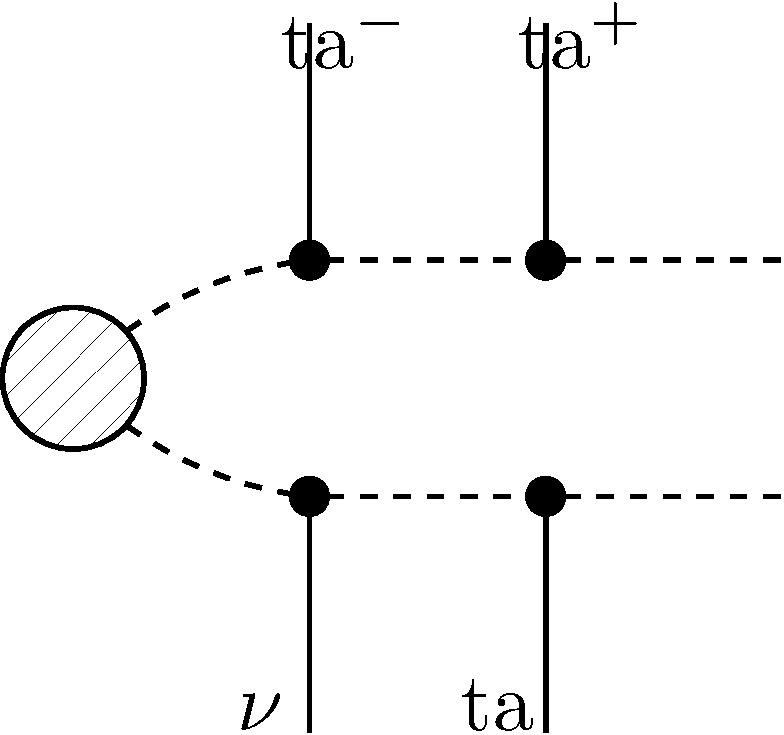
\includegraphics[width=0.15\linewidth]{figures/ATLAS_CONF_2013_028:TChiChipmStauL_TChiChipmStauL_3_.pdf}\spacer+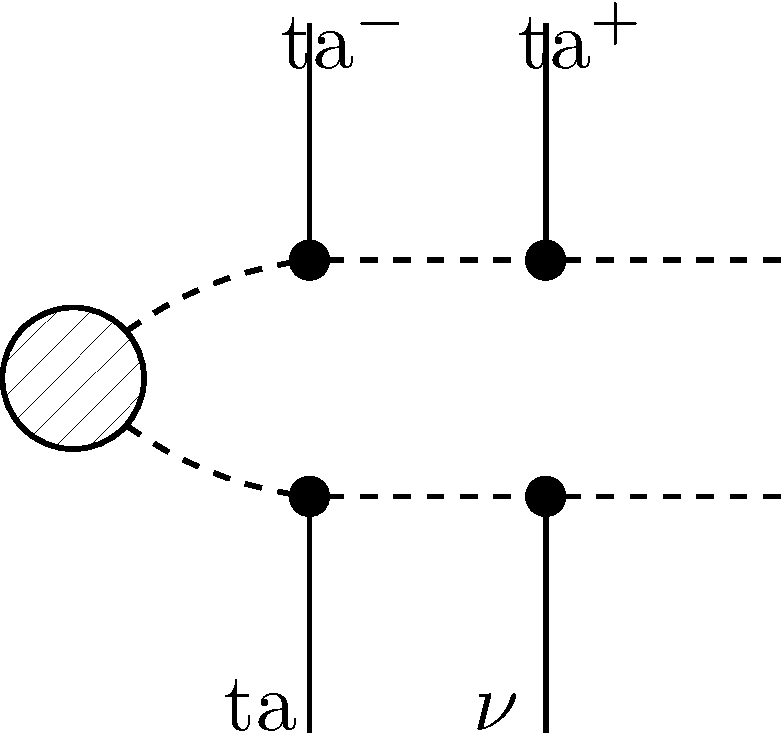
\includegraphics[width=0.15\linewidth]{figures/ATLAS_CONF_2013_028:TChiChipmStauL_TChiChipmStauL_4_.pdf}\spacer) \\ 
 &  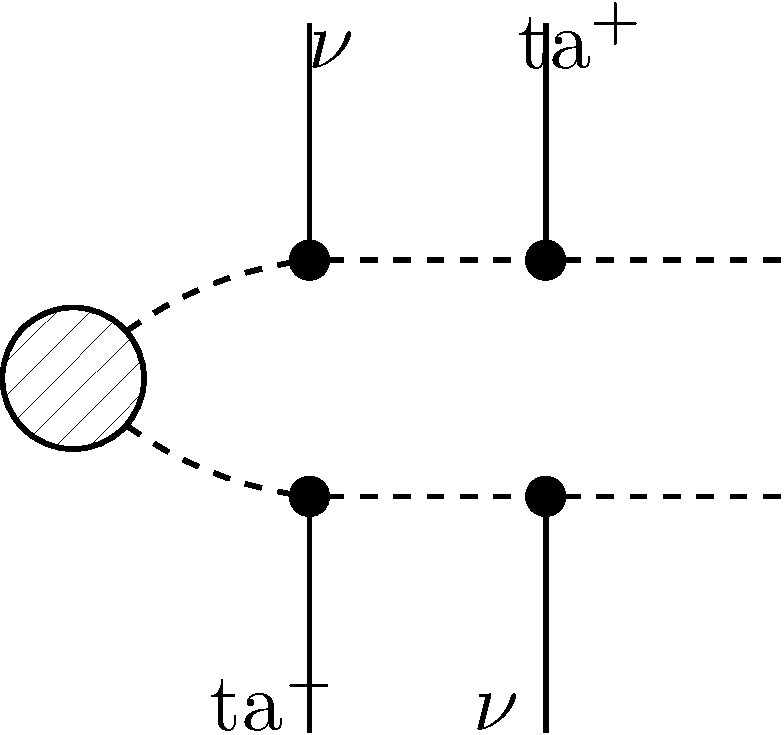
\includegraphics[width=0.15\linewidth]{figures/ATLAS_CONF_2013_028:TChipChimStauSnu_TChipChimStauSnu_1_.pdf}\spacer+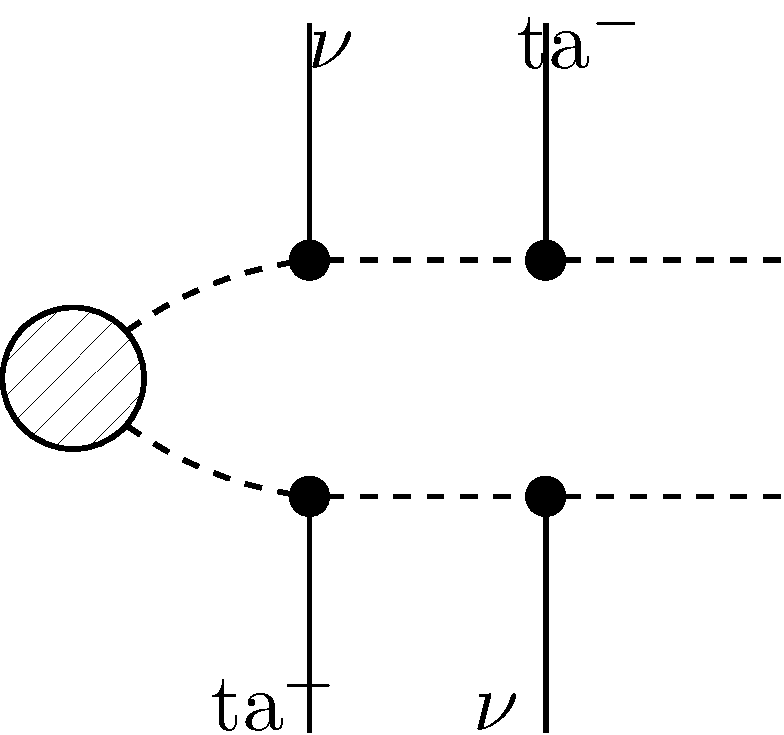
\includegraphics[width=0.15\linewidth]{figures/ATLAS_CONF_2013_028:TChipChimStauSnu_TChipChimStauSnu_2_.pdf}\spacer+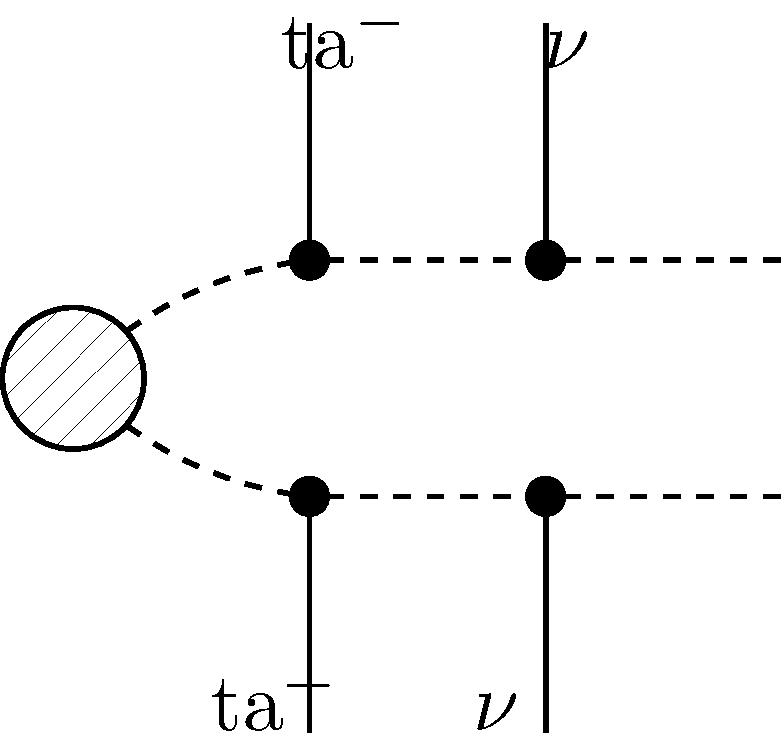
\includegraphics[width=0.15\linewidth]{figures/ATLAS_CONF_2013_028:TChipChimStauSnu_TChipChimStauSnu_3_.pdf}\spacer+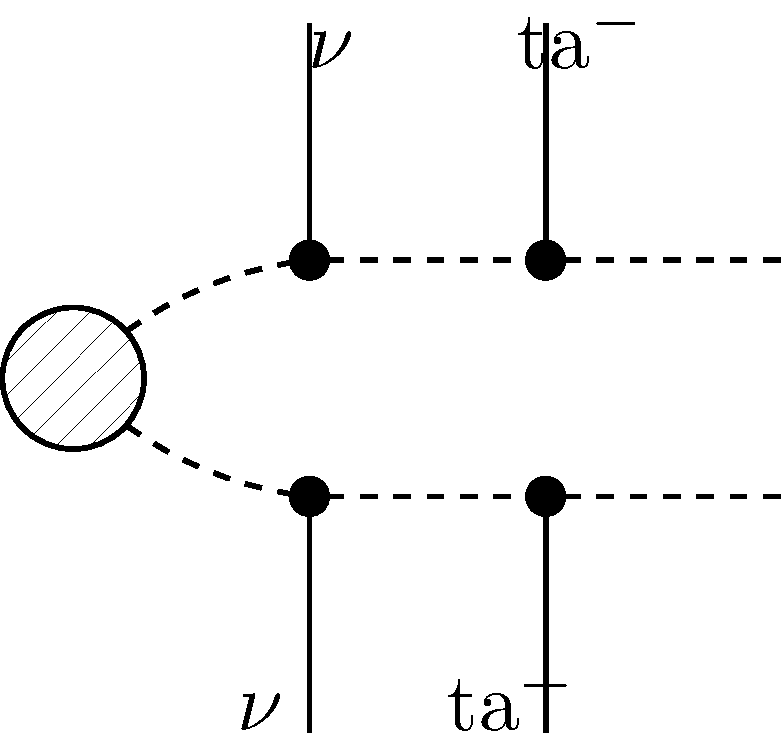
\includegraphics[width=0.15\linewidth]{figures/ATLAS_CONF_2013_028:TChipChimStauSnu_TChipChimStauSnu_4_.pdf}\spacer \\  \hline 
\multirow{6}{*}{Weakinos8TeV } &  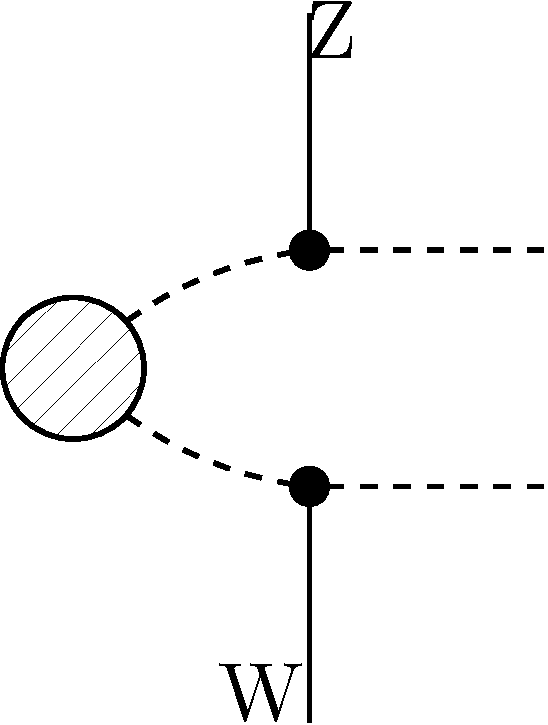
\includegraphics[width=0.15\linewidth]{figures/Weakinos8TeV:TChiWZ_TChiWZ_1_.pdf}\spacer \\ 
 &  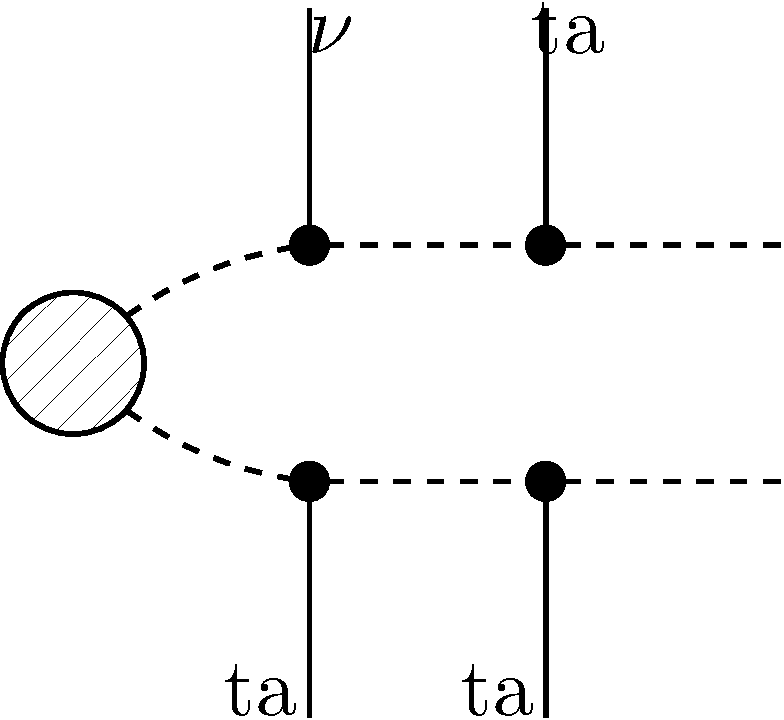
\includegraphics[width=0.15\linewidth]{figures/Weakinos8TeV:TChiChipmStauStau_TChiChipmStauStau_1_.pdf}\spacer \\ 
 &  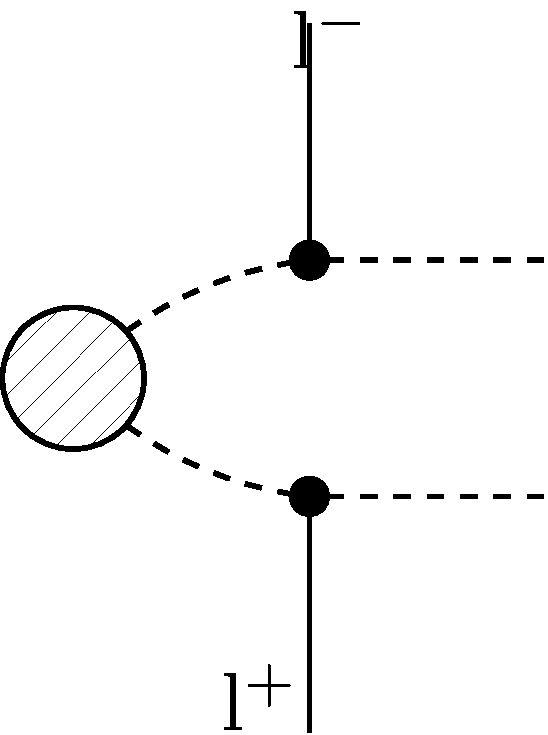
\includegraphics[width=0.15\linewidth]{figures/Weakinos8TeV:TSlepSlep_TSlepSlep_1_.pdf}\spacer \\ 
 &  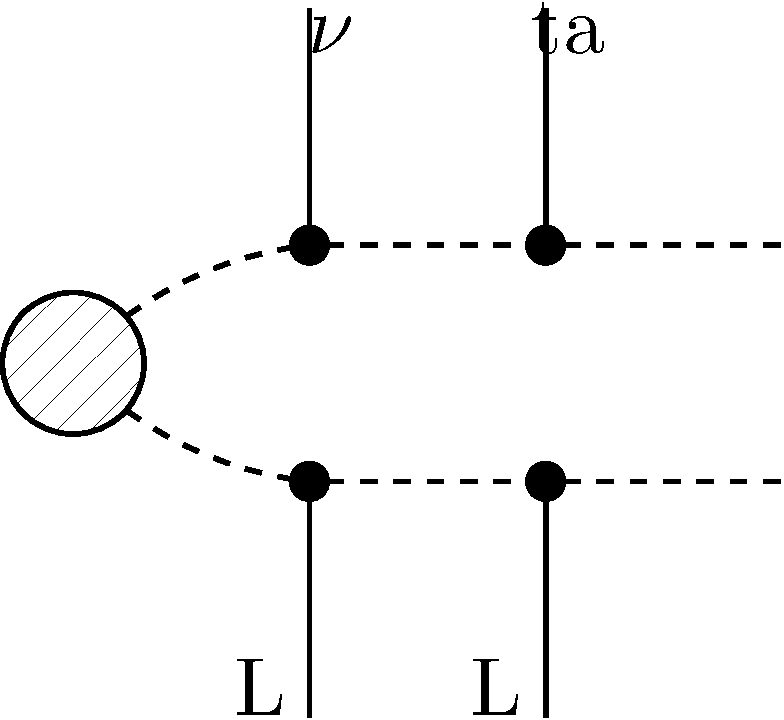
\includegraphics[width=0.15\linewidth]{figures/Weakinos8TeV:TChiChipmSlepStau_TChiChipmSlepStau_1_.pdf}\spacer \\ 
 &  2.*(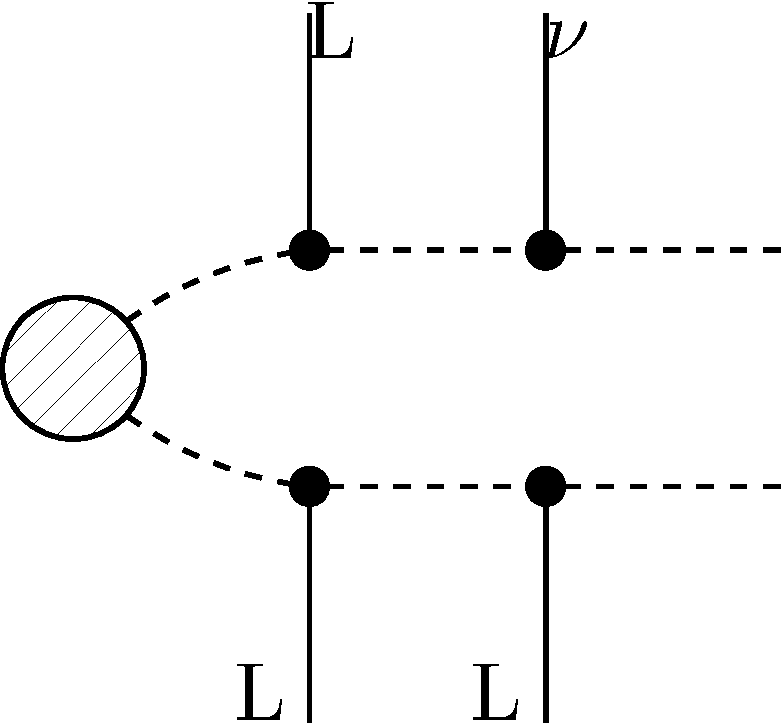
\includegraphics[width=0.15\linewidth]{figures/Weakinos8TeV:TChiChipmSlepL_TChiChipmSlepL_1_.pdf}\spacer+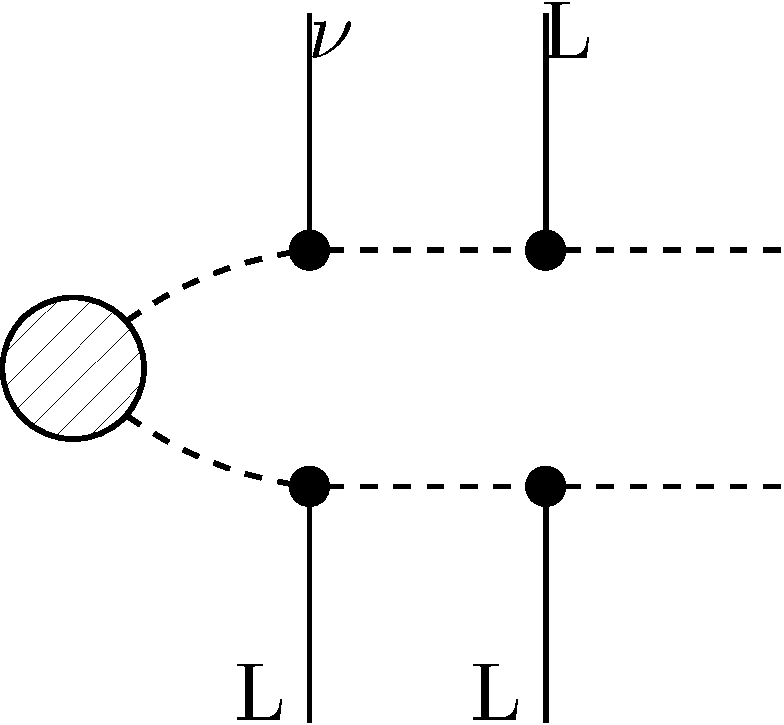
\includegraphics[width=0.15\linewidth]{figures/Weakinos8TeV:TChiChipmSlepL_TChiChipmSlepL_2_.pdf}\spacer) \\ 
 &  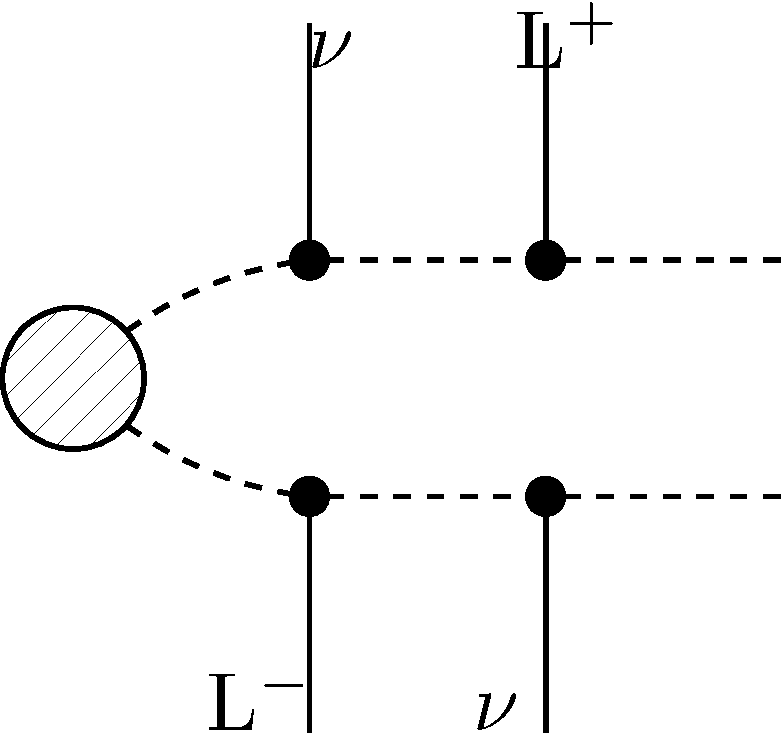
\includegraphics[width=0.15\linewidth]{figures/Weakinos8TeV:TChipChimSlepSnu_TChipChimSlepSnu_1_.pdf}\spacer+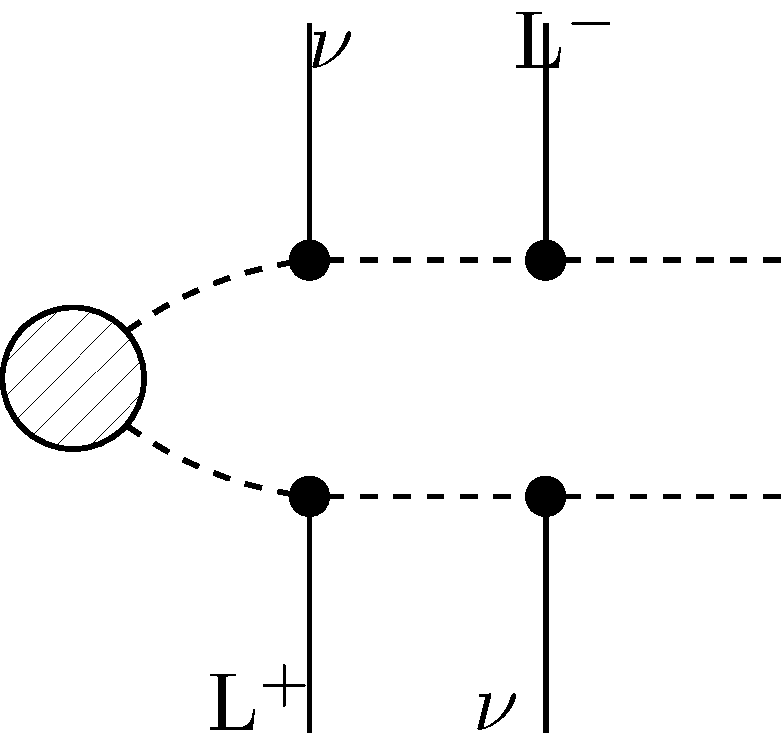
\includegraphics[width=0.15\linewidth]{figures/Weakinos8TeV:TChipChimSlepSnu_TChipChimSlepSnu_2_.pdf}\spacer+\includegraphics[width=0.15\linewidth]{figures/Weakinos8TeV:TChipChimSlepSnu_TChipChimSlepSnu_3_.pdf}\spacer+\includegraphics[width=0.15\linewidth]{figures/Weakinos8TeV:TChipChimSlepSnu_TChipChimSlepSnu_4_.pdf}\spacer \\  \hline 
\multirow{5}{*}{SUS13008 } &  \includegraphics[width=0.15\linewidth]{figures/SUS13008:T6ttWW_T6ttWW_1_.pdf}\spacer \\ 
 &  \includegraphics[width=0.15\linewidth]{figures/SUS13008:T1tttt_T1tttt_1_.pdf}\spacer \\ 
 &  \includegraphics[width=0.15\linewidth]{figures/SUS13008:T6bbZZ_T6bbZZ_1_.pdf}\spacer \\ 
 &  \includegraphics[width=0.15\linewidth]{figures/SUS13008:T7btbtWW_T7btbtWW_1_.pdf}\spacer \\ 
 &  \includegraphics[width=0.15\linewidth]{figures/SUS13008:T5tttt_T5tttt_1_.pdf}\spacer \\  \hline 
\multirow{2}{*}{RA2b8TeV } &  \includegraphics[width=0.15\linewidth]{figures/RA2b8TeV:T1bbbb_T1bbbb_1_.pdf}\spacer \\ 
 &  \includegraphics[width=0.15\linewidth]{figures/RA2b8TeV:T1tttt_T1tttt_1_.pdf}\spacer \\  \hline 
\multirow{6}{*}{alphaT8TeV } &  \includegraphics[width=0.15\linewidth]{figures/alphaT8TeV:T1bbbb_T1bbbb_1_.pdf}\spacer \\ 
 &  \includegraphics[width=0.15\linewidth]{figures/alphaT8TeV:T2tt_T2tt_1_.pdf}\spacer \\ 
 &  \includegraphics[width=0.15\linewidth]{figures/alphaT8TeV:T1tttt_T1tttt_1_.pdf}\spacer \\ 
 &  \includegraphics[width=0.15\linewidth]{figures/alphaT8TeV:T2_T2_1_.pdf}\spacer \\ 
 &  \includegraphics[width=0.15\linewidth]{figures/alphaT8TeV:T1_T1_1_.pdf}\spacer \\ 
 &  \includegraphics[width=0.15\linewidth]{figures/alphaT8TeV:T2bb_T2bb_1_.pdf}\spacer \\  \hline 
\multirow{1}{*}{ATLAS-CONF-2012-105 } &  \includegraphics[width=0.15\linewidth]{figures/ATLAS_CONF_2012_105:T1tttt_T1tttt_1_.pdf}\spacer \\  \hline 
\multirow{1}{*}{RA48TeV } &  \includegraphics[width=0.15\linewidth]{figures/RA48TeV:T1tttt_T1tttt_1_.pdf}\spacer \\  \hline 
\caption{LHC analyses included in our results. We also show the SMS topologies (or sums of topologies) constrained by each analysis\fixme{Just a rough idea.Definetely needs improvement}.} 
   \label{tab:LHCresults} 
   \end{longtable}

\FloatBarrier


\end{appendix}


\bibliography{references}

\end{document}

